\chapter{Curves}\label{chap:curves}

% ==================== Section 1-1: Introduction ====================
\section{Introduction}\label{sec:intro}

\textbf{The problem we face.} 我们生活在一个三维空间中，而视觉是我们感知世界的主要方式之一。当我们观察一条曲线——无论是一条道路、一条河流的轮廓、还是行星在天空中的运动轨迹——我们的大脑本能地识别它的"弯曲程度"。这种对弯曲的直观感知，引导我们提出一个根本性的问题：

\textit{如何用精确的数学语言来描述曲线的弯曲程度？}

这个问题看似简单，却贯穿了整个微分几何的发展历程。从欧几里得几何中直线与圆的基本定义，到高斯研究曲面的内在几何，再到达布（Darboux）建立曲线与曲面的局部理论，这个问题的答案逐渐清晰：曲线的弯曲程度可以通过其在一点处的加速度来度量。

\textbf{The main theme.} 微分几何研究的是曲线和曲面的几何性质。与微积分研究函数变化不同，微分几何关注的是空间中曲线和曲面的"形状"——弯曲程度、扭曲程度等内在几何量。

经典微分几何始于微积分诞生之时，其核心是研究曲线和曲面的\textbf{局部性质}（local properties）——即那些仅依赖于曲线或曲面在一点附近行为的几何性质。使用的工具正是微分计算。我们将会看到，一个出人意料的事实是：空间曲线的形状完全由两个函数决定——曲率（curvature）和挠率（torsion）。

\textbf{A guiding example.} 在学习曲线的理论时，一个例子将贯穿始终，这就是圆柱螺旋线（cylindrical helix）。想象一条弹簧从空中掉落，它在空中划出的轨迹就是螺旋线。螺旋线的非凡之处在于：它在弯曲的同时保持恒定的扭转率。这种"均匀弯曲 + 均匀扭曲"的特性，使其成为理解曲率与挠率概念的完美载体。

\textbf{Organization of this chapter.} 本章的组织方式如下。1-2 节到 1-4 节包含基础内容（参数曲线、弧长、向量积），可作为复习；1-5 节是核心，引入曲率和挠率的概念；1-6 节和 1-7 节讨论局部标准形式和整体性质。若只想学习曲面，可以跳过 1-6、1-7 节。

\begin{figure}[H]
\centering
\begin{minipage}{0.45\textwidth}
\centering
\subfloat[Figure 1-1. 圆柱螺旋线 (helix) — 弯曲与扭曲的完美结合]{\label{fig:helix}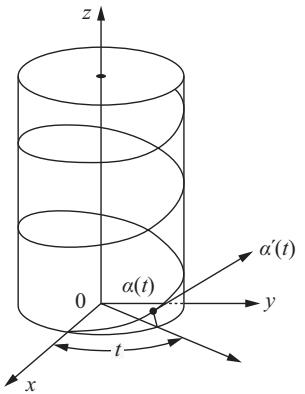
\includegraphics[width=\textwidth]{../../../PDFs/differential-geometry/transcript/Do Carmo - Differential Geometry of Curves and Surfaces/hybrid_ocr/images/1368896b0e1df27036554e8c66d6bc05c3fbc6b6c2bca19cecb0d396544dfb0a.jpg}}
\end{minipage}
\hfill
\begin{minipage}{0.50\textwidth}
\centering
\subfloat[Figure 1-2. 奇异点例子 — 曲线在尖点处不可微]{\label{fig:trace1}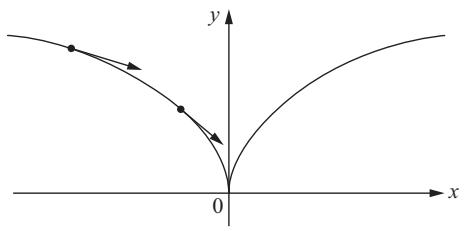
\includegraphics[width=\textwidth]{../../../PDFs/differential-geometry/transcript/Do Carmo - Differential Geometry of Curves and Surfaces/hybrid_ocr/images/fe1d17628a3c9bb1e6afbeeae0fdac47edd92f0cb4651af800c230be43509433.jpg}}
\end{minipage}
\end{figure}

\begin{figure}[H]
\centering
\begin{minipage}{0.60\textwidth}
\centering
\subfloat[Figure 1-3. 非单射曲线例子 — 同一点被多次经过]{\label{fig:trace2}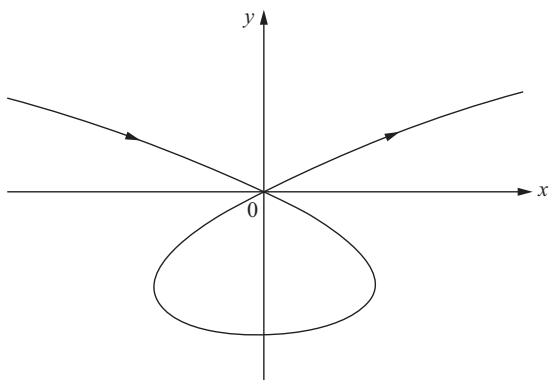
\includegraphics[width=\textwidth]{../../../PDFs/differential-geometry/transcript/Do Carmo - Differential Geometry of Curves and Surfaces/hybrid_ocr/images/cb0e93ccd913afbcf8adab5178a99f0ac4808db3b32ad2dbe4971ce9b314a9aa.jpg}}
\end{minipage}
\end{figure}

% ==================== Section 1-2: Parametrized Curves ====================
\section{Parametrized Curves}\label{sec:parametrized-curves}

\textbf{Why parametrization?} 在我们提出"如何描述曲线的弯曲程度"这个问题之后，自然的下一步是找到描述曲线的数学工具。我们已经知道，微积分是研究函数变化的有力武器——那么，是否可以将曲线视为某种"函数"，从而运用微分学的工具？

这个想法引导我们引入\textbf{参数化}的概念。其核心思想简单而优雅：将曲线看作一个从区间到空间的映射。例如，当我们说"质点沿曲线运动"时，时间 $t$ 是参数，位置 $\alpha(t)$ 是 $t$ 的函数。这种视角不仅统一了古代对圆、椭圆等特殊曲线的研究，更为重要的是，它让我们能够使用导数来研究曲线的局部几何性质。

接下来，我们首先回顾 $\mathbb{R}^3$ 中向量内积的基本性质，这对后续讨论至关重要。

\begin{Remark}
设 $u = (u_1, u_2, u_3) \in \mathbb{R}^3$，定义其范数（或长度）为
\[
|u| = \sqrt{u_1^2 + u_2^2 + u_3^2}.
\]
几何上，$|u|$ 是点 $(u_1, u_2, u_3)$ 到原点 $O = (0, 0, 0)$ 的距离。

设 $u = (u_1, u_2, u_3)$ 和 $v = (v_1, v_2, v_3)$ 是 $\mathbb{R}^3$ 中的向量，$\theta$ ($0 \leq \theta \leq \pi$) 是线段 $Ou$ 和 $Ov$ 之间的夹角。内积 $u \cdot v$ 定义为（教材 Figure 1-6（见 \cref{fig:fig1-6}））：
\[
u \cdot v = |u| |v| \cos\theta.
\]

内积的基本性质：
\begin{enumerate}
\item 若 $u$ 和 $v$ 为非零向量，则 $u \cdot v = 0$ 当且仅当 $u$ 与 $v$ 正交；
\item $u \cdot v = v \cdot u$；
\item $\lambda(u \cdot v) = \lambda u \cdot v = u \cdot \lambda v$；
\item $u \cdot (v + w) = u \cdot v + u \cdot w$。
\end{enumerate}
\end{Remark}

\begin{figure}[H]
\centering
\begin{minipage}{0.7\textwidth}
\centering
\subfloat[Figure 1-6. 内积的几何意义]{\label{fig:fig1-6}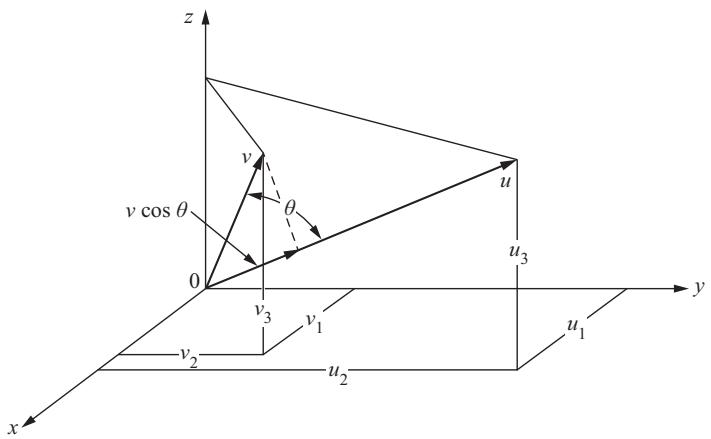
\includegraphics[width=\textwidth]{../../../PDFs/differential-geometry/transcript/Do Carmo - Differential Geometry of Curves and Surfaces/hybrid_ocr/images/a0b92278a00bbcb50d6fd77bfcf8714675cdfc630be2b734b1bf7849214de53e.jpg}}
\end{minipage}
\end{figure}

\textbf{The central notion.} 我们用 $\mathbb{R}^3$ 表示所有三元实数有序组 $(x, y, z)$ 的集合。现在，我们正式引入参数化曲线的概念。

\begin{Definition}[可微参数曲线]\label{def:parametrized-curve}
\textbf{可微参数曲线}是一个可微映射
\[
\alpha: \mathbf{I} \to \mathbb{R}^3,
\]
其中 $\mathbf{I} = (\mathbf{a}, \mathbf{b})$ 是实数直线 $\mathbb{R}$ 上的一个开区间。
\end{Definition}

可微意味着 $\alpha$ 将每个 $t \in I$ 映射到点 $\alpha(t) = (x(t), y(t), z(t)) \in \mathbb{R}^3$，其中函数 $x(t), y(t), z(t)$ 都是可微的。变量 $t$ 称为曲线的\textbf{参数}。

如果记 $x(t)$ 在 $t$ 处的一阶导数为 $x'(t)$，等等，则向量
\[
(x'(t), y'(t), z'(t)) = \alpha'(t) \in \mathbb{R}^3
\]
称为曲线 $\alpha$ 在 $t$ 处的\textbf{切向量}（tangent vector）或\textbf{速度向量}（velocity vector）。像集 $\alpha(I) \subset \mathbb{R}^3$ 称为 $\alpha$ 的\textbf{迹}（trace）。如下面的例 5 所示，我们必须注意区分参数曲线（它是一个映射）和它的迹（它是 $\mathbb{R}^3$ 的一个子集）。

\begin{Remark}
术语说明：许多人用"无限可微"来表示具有各阶导数（且自动连续）的函数，而用"可微"仅表示一阶导数的存在性。我们不采用这种用法——本书中"可微"意味着所有阶导数都存在。
\end{Remark}

\textbf{Examples.} 为了建立直觉，我们来看几个关键的例子，它们将贯穿本章的讨论。

\begin{figure}[H]
\centering
\begin{minipage}{0.40\textwidth}
\centering
\subfloat[Figure 1-1. 圆柱螺旋线 (helix)]{\label{fig:helix-example}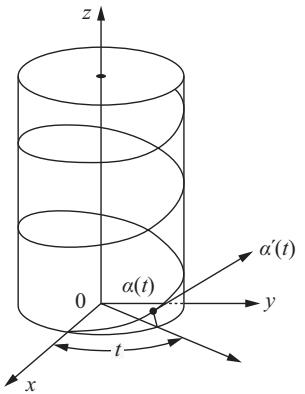
\includegraphics[width=\textwidth]{../../../PDFs/differential-geometry/transcript/Do Carmo - Differential Geometry of Curves and Surfaces/hybrid_ocr/images/1368896b0e1df27036554e8c66d6bc05c3fbc6b6c2bca19cecb0d396544dfb0a.jpg}}
\end{minipage}
\hfill
\begin{minipage}{0.50\textwidth}
\centering
\subfloat[Figure 1-2. 奇异点例子]{\label{fig:trace1-example}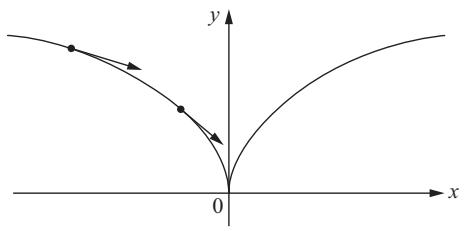
\includegraphics[width=\textwidth]{../../../PDFs/differential-geometry/transcript/Do Carmo - Differential Geometry of Curves and Surfaces/hybrid_ocr/images/fe1d17628a3c9bb1e6afbeeae0fdac47edd92f0cb4651af800c230be43509433.jpg}}
\end{minipage}
\end{figure}

\begin{Example}[圆柱螺旋线]\label{ex:helix}
参数方程
\[
\alpha(t) = (a\cos t,\; a\sin t,\; bt),\quad t \in \mathbb{R}
\]
在 $\mathbb{R}^3$ 中的迹是圆柱面 $x^2 + y^2 = a^2$ 上的螺旋线（helix），螺距（pitch）为 $2\pi b$。这里参数 $t$ 测量的是 $x$ 轴与从原点 $O$ 到点 $\alpha(t)$ 在 $xy$ 平面上投影点的连线之间的夹角（教材 Figure 1-1（见 \cref{fig:helix-example}））。
\end{Example}

正如本章引言所述，螺旋线将成为我们理解曲率与挠率的完美载体——它的"均匀弯曲 + 均匀扭曲"特性，使其在后续讨论中反复出现。

\begin{Example}[奇异点]\label{ex:singular-point}
映射 $\alpha: \mathbb{R} \to \mathbb{R}^2$，$\alpha(t) = (t^3, t^2)$，是一条可微参数曲线（教材 Figure 1-2（见 \cref{fig:trace1-example}））。注意 $\alpha'(0) = (0, 0)$——即 $t = 0$ 处的速度向量为零。这样的点称为\textbf{奇异点}（singular point）。

奇异点的出现提醒我们：可微的参数方程并不保证曲线在每一点都有"良好"的行为。
\end{Example}

\begin{figure}[H]
\centering
\begin{minipage}{0.60\textwidth}
\centering
\subfloat[Figure 1-3. 非单射曲线例子]{\label{fig:trace2-example}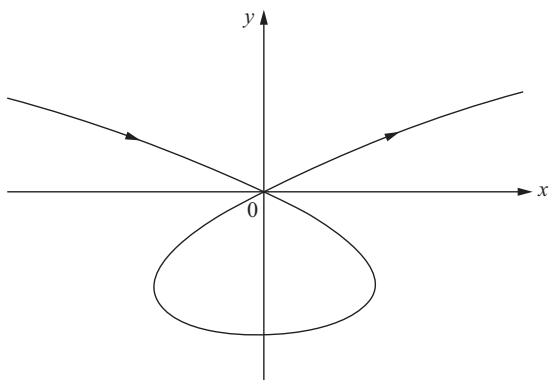
\includegraphics[width=\textwidth]{../../../PDFs/differential-geometry/transcript/Do Carmo - Differential Geometry of Curves and Surfaces/hybrid_ocr/images/cb0e93ccd913afbcf8adab5178a99f0ac4808db3b32ad2dbe4971ce9b314a9aa.jpg}}
\end{minipage}
\end{figure}

\begin{Example}[非单射曲线]\label{ex:non-injective}
映射 $\alpha: \mathbb{R} \to \mathbb{R}^2$，$\alpha(t) = (t^3 - 4t,\; t^2 - 4)$，是一条可微参数曲线（教材 Figure 1-3（见 \cref{fig:trace2-example}））。注意 $\alpha(2) = \alpha(-2) = (0, 0)$——即映射 $\alpha$ 不是单射。

这个例子说明一个重要事实：参数化与曲线本身是不同的概念。同一条曲线可以有多种参数化方式。
\end{Example}

\begin{Example}[不可微曲线]\label{ex:nondifferentiable}
映射 $\alpha: \mathbb{R} \to \mathbb{R}^2$，$\alpha(t) = (t, |t|)$，$t \in \mathbb{R}$，不是可微参数曲线，因为 $|t|$ 在 $t = 0$ 处不可微（教材 Figure 1-4（见 \cref{fig:fig1-4}））。

这个例子表明我们的定义排除了"带尖角"的曲线——这正是微分几何研究平滑曲线的自然选择。
\end{Example}

\begin{figure}[H]
\centering
\begin{minipage}{0.55\textwidth}
\centering
\subfloat[Figure 1-4. 不可微曲线 $(t, |t|)$]{\label{fig:fig1-4}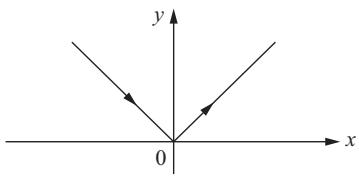
\includegraphics[width=\textwidth]{../../../PDFs/differential-geometry/transcript/Do Carmo - Differential Geometry of Curves and Surfaces/hybrid_ocr/images/3ccb4fd7f5ebe66c541905ee2202d214dc1c8d2d699dace1fe66d0754f0bba7d.jpg}}
\end{minipage}
\hfill
\begin{minipage}{0.40\textwidth}
\centering
\subfloat[Figure 1-5. 相同圆的不同参数化]{\label{fig:fig1-5}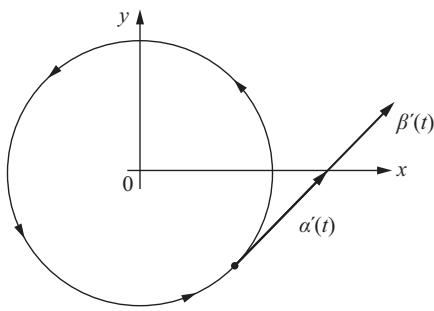
\includegraphics[width=\textwidth]{../../../PDFs/differential-geometry/transcript/Do Carmo - Differential Geometry of Curves and Surfaces/hybrid_ocr/images/5c1a7770e5c0b4bfc9eab7055561b6a0abd1f5782eb7ecbdebd9abcbd5977fe3.jpg}}
\end{minipage}
\end{figure}

\begin{Example}[相同迹的不同参数化]\label{ex:same-trace-different-param}
两条不同的参数曲线
\[
\alpha(t) = (\cos t, \sin t),\quad \beta(t) = (\cos 2t, \sin 2t),
\]
其中 $t \in (-\epsilon, 2\pi + \epsilon)$，$\epsilon > 0$，具有相同的迹——即单位圆 $x^2 + y^2 = 1$。但第二条曲线的速度向量是第一条的两倍（教材 Figure 1-5（见 \cref{fig:fig1-5}））。

这引出一个关键观察：曲线的"形状"（迹）与描述它的"方式"（参数化）是不同的概念。这种区别在后续引入弧长参数化时将变得尤为重要。
\end{Example}

\subsection*{1-2 节练习}

\begin{exercise}{1-2, 1 — do Carmo, Exercise 1-2, 1}
Find a parametrized curve $\alpha(t)$ whose trace is the circle $x^2 + y^2 = 1$ such that $\alpha(t)$ runs clockwise around the circle with $\alpha(0) = (0, 1)$.
\end{exercise}

\begin{exercise}{1-2, 2 — do Carmo, Exercise 1-2, 2}
Let $\alpha(t)$ be a parametrized curve which does not pass through the origin. If $\alpha(t_0)$ is a point of the trace of $\alpha$ closest to the origin and $\alpha'(t_0) \neq 0$, show that the position vector $\alpha(t_0)$ is orthogonal to $\alpha'(t_0)$.
\end{exercise}

\begin{exercise}{1-2, 3 — do Carmo, Exercise 1-2, 3}
A parametrized curve $\alpha(t)$ has the property that its second derivative $\alpha''(t)$ is identically zero. What can be said about $\alpha$?
\end{exercise}

\begin{exercise}{1-2, 4 — do Carmo, Exercise 1-2, 4}
Let $\alpha: I \to \mathbb{R}^3$ be a parametrized curve and let $v \in \mathbb{R}^3$ be a fixed vector. Assume that $\alpha'(t)$ is orthogonal to $v$ for all $t \in I$ and that $\alpha(0)$ is also orthogonal to $v$. Prove that $\alpha(t)$ is orthogonal to $v$ for all $t \in I$.
\end{exercise}

\begin{exercise}{1-2, 5 — do Carmo, Exercise 1-2, 5}
Let $\alpha: I \to \mathbb{R}^3$ be a parametrized curve, with $\alpha'(t) \neq 0$ for all $t \in I$. Show that $|\alpha(t)|$ is a nonzero constant if and only if $\alpha(t)$ is orthogonal to $\alpha'(t)$ for all $t \in I$.
\end{exercise}

% ==================== Section 1-3: Regular Curves; Arc Length ====================
\section{Regular Curves; Arc Length}\label{sec:regular-arc-length}

\textbf{The need for regular curves.} 当我们引入参数化曲线的概念后，自然会问：是否每个可微参数曲线都能用微分学的工具来研究？

答案并非总是肯定的。我们已经看到，奇异点（如 $\alpha(t) = (t^3, t^2)$ 在 $t=0$ 处）的出现会导致切向量为零，这会给后续的微分运算带来麻烦。更根本的是：如果 $\alpha'(t) = 0$，那么在该点处就不存在确定的切线——这对于研究曲线的"弯曲程度"是致命的。

因此，在研究曲线的微分几何时，我们必须把注意力限制在每一点都有良好定义的切线的曲线上。这引导我们引入正则曲线的概念。

设 $\alpha: I \to \mathbb{R}^3$ 是一条可微参数曲线。对于每个满足 $\alpha'(t) \neq 0$ 的 $t \in I$，存在一条唯一定义直线，它经过点 $\alpha(t)$ 且与向量 $\alpha'(t)$ 平行。这条直线称为曲线 $\alpha$ 在 $t$ 处的\textbf{切线}（tangent line）。

\begin{Definition}[正则曲线]\label{def:regular-curve}
如果 $\alpha'(t) \neq 0$ 对所有 $t \in \mathbf{I}$ 成立，则称可微参数曲线 $\alpha: \mathbf{I} \to \mathbb{R}^3$ 为\textbf{正则曲线}（regular curve）。
\end{Definition}

\textbf{Why arc length?} 在有了正则曲线的概念之后，我们转向一个更基本的问题：如何测量曲线的长度？

这个问题看似简单，却揭示了微分几何的一个核心思想。直观上，曲线的长度应该是其"内在"属性——它不应该依赖于我们如何参数化这条曲线。果真如此吗？

答案是肯定的，这正是弧长公式的非凡之处。

\begin{Definition}[弧长]\label{def:arc-length}
设 $\alpha: [a,b] \to \mathbb{R}^3$ 是一条可微曲线。$\alpha$ 从 $t = a$ 到 $t$ 的\textbf{弧长}（arc length）定义为
\[
s(t) = \int_a^t \|\alpha'(u)\| \, du.
\]
\end{Definition}

弧长是曲线的内在不变量，与参数化选择无关。

\begin{figure}[H]
\centering
\begin{minipage}{0.85\textwidth}
\centering
\subfloat[Figure 1-7. 旋轮线 (cycloid)]{\label{fig:cycloid}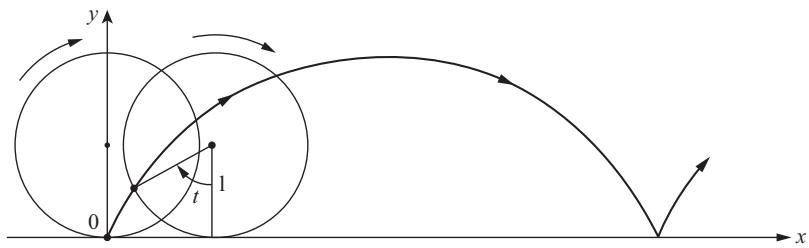
\includegraphics[width=\textwidth]{../../../PDFs/differential-geometry/transcript/Do Carmo - Differential Geometry of Curves and Surfaces/hybrid_ocr/images/63bc08d607172bd6a8b21cbb1b3d77d9488cb451250e9185505320fee946bdea.jpg}}
\end{minipage}
\end{figure}

\begin{figure}[H]
\centering
\begin{minipage}{0.35\textwidth}
\centering
\subfloat[Figure 1-8. Diocles 割舌线 (cissoid)]{\label{fig:cissoid}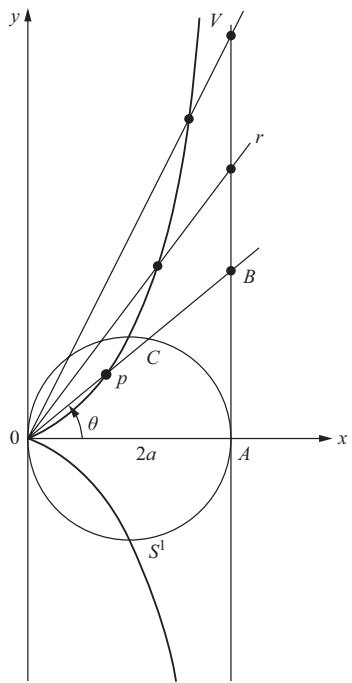
\includegraphics[width=\textwidth]{../../../PDFs/differential-geometry/transcript/Do Carmo - Differential Geometry of Curves and Surfaces/hybrid_ocr/images/7cb4e48e7dffd2801d004ed55334f427682431254e840be3a0f41770ff7e5f4b.jpg}}
\end{minipage}
\hfill
\begin{minipage}{0.30\textwidth}
\centering
\subfloat[Figure 1-9. 曳物线 (tractrix)]{\label{fig:tractrix}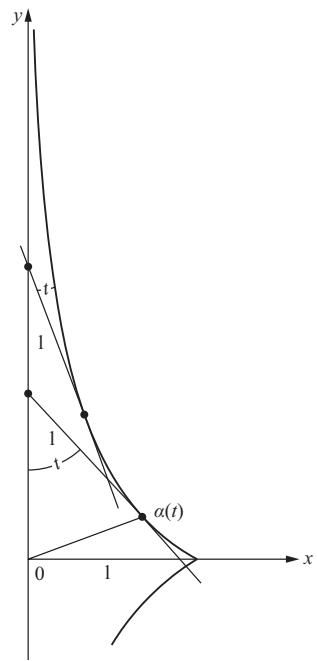
\includegraphics[width=\textwidth]{../../../PDFs/differential-geometry/transcript/Do Carmo - Differential Geometry of Curves and Surfaces/hybrid_ocr/images/ce65cd4c5b99c388091efe63d303bf387148984fd4d56aa49e7df3e7ecee7b8b.jpg}}
\end{minipage}
\end{figure}

\begin{Proposition}[弧长参数化]\label{prop:arc-length-reparam}
设 $\alpha: I \to \mathbb{R}^3$ 是正则曲线。定义
\[
s(t) = \int_{t_0}^t \|\alpha'(u)\| \, du,
\]
其中 $t_0 \in I$ 是固定点。由于 $\alpha$ 是正则的，$s'(t) = \|\alpha'(t)\| > 0$，所以 $s$ 是严格递增的，可以取逆函数 $t(s)$。则 $\beta(s) = \alpha(t(s))$ 是单位速度曲线。
\end{Proposition}

\begin{Definition}[单位速度曲线]\label{def:unit-speed}
如果 $\|\alpha'(t)\| = 1$ 对所有 $t$ 成立，则称 $\alpha$ 为\textbf{单位速度曲线}（unit speed curve）或\textbf{弧长参数化曲线}。
\end{Definition}

从现在开始，除非特别说明，我们将使用弧长 $s$ 作为参数，即 $\alpha(s)$ 是单位速度曲线。

\begin{Remark}
弧长参数化后，速度向量恒为 $1$，这是最自然的参数化方式。此时 $\alpha'(s)$ 是单位切向量。
\end{Remark}

\begin{Example}[圆的弧长]\label{ex:circle-arc-length}
半径为 $a$ 的圆可以参数化为 $\alpha(t) = (a\cos t, a\sin t, 0)$，$t \in [0, 2\pi]$。则弧长
\[
s(t) = \int_0^t \|\alpha'(u)\| \, du = \int_0^t a \, du = at,
\]
所以从 $t = 0$ 到 $t = 2\pi$ 的全长是 $2\pi a$。
\end{Example}

\begin{Example}[圆柱螺旋线的弧长]\label{ex:helix-arc-length}
圆柱螺旋线 $\alpha(t) = (a\cos t, a\sin t, bt)$ 的速度向量为 $\alpha'(t) = (-a\sin t, a\cos t, b)$，模长为
\[
\|\alpha'(t)\| = \sqrt{a^2 + b^2}.
\]
因此弧长为 $s(t) = \sqrt{a^2 + b^2}\, t$。
\end{Example}

\begin{figure}[H]
\centering
\begin{minipage}{0.45\textwidth}
\centering
\subfloat[Figure 1-10. 笛卡尔叶形线 (folium of Descartes)]{\label{fig:folium}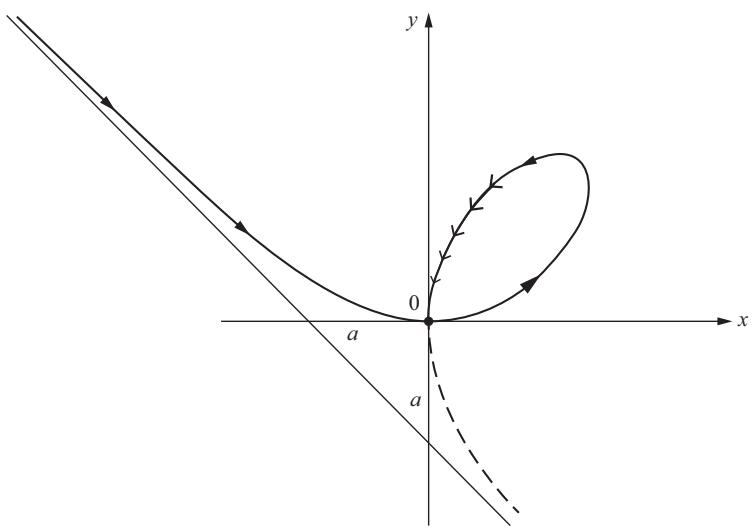
\includegraphics[width=\textwidth]{../../../PDFs/differential-geometry/transcript/Do Carmo - Differential Geometry of Curves and Surfaces/hybrid_ocr/images/53989c2c8bd35e9940d7e50e2d083d788a381c25ec567919134018f0aa652a4a.jpg}}
\end{minipage}
\hfill
\begin{minipage}{0.45\textwidth}
\centering
\subfloat[Figure 1-11. 对数螺旋线 (logarithmic spiral)]{\label{fig:log-spiral}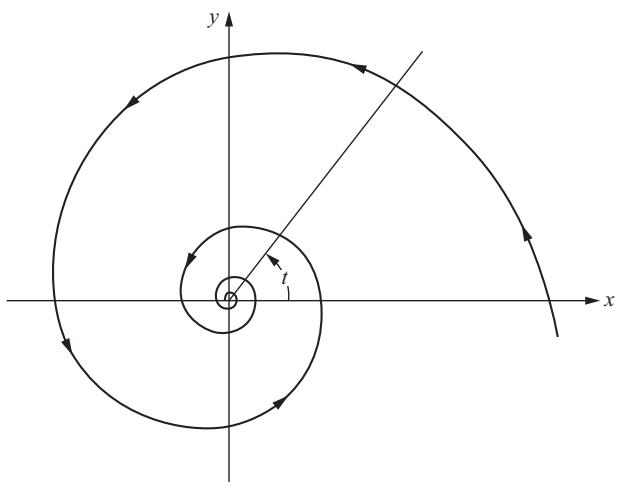
\includegraphics[width=\textwidth]{../../../PDFs/differential-geometry/transcript/Do Carmo - Differential Geometry of Curves and Surfaces/hybrid_ocr/images/2174ba1ba51fc162114661ee328aff35710e3764b7c59adb18400b0b6598d634.jpg}}
\end{minipage}
\end{figure}

\subsection*{1-3 节练习}

\begin{exercise}{1-3, 1 — do Carmo, Exercise 1-3, 1}
Show that the tangent lines to the regular parametrized curve $\alpha(t) = (3t, 3t^2, 2t^3)$ make a constant angle with the line $y = 0,\; z = x$.
\end{exercise}

\begin{exercise}{1-3, 2 — do Carmo, Exercise 1-3, 2}
A circular disk of radius 1 in the plane $xy$ rolls without slipping along the $x$ axis. The figure described by a point of the circumference of the disk is called a cycloid (see \cref{fig:cycloid}, do Carmo, Figure 1-7).
\begin{enumerate}
\item[a.] Obtain a parametrized curve $\alpha: \mathbb{R} \to \mathbb{R}^2$ the trace of which is the cycloid, and determine its singular points.
\item[b.] Compute the arc length of the cycloid corresponding to a complete rotation of the disk.
\end{enumerate}
\end{exercise}

\begin{exercise}{1-3, 3 — do Carmo, Exercise 1-3, 3}
Let $0A = 2a$ be the diameter of a circle $S^1$. Prove that:
\begin{enumerate}
\item[a.] The trace of
\[
\alpha(t) = \left(\frac{2at^2}{1+t^2}, \frac{2at^3}{1+t^2}\right),\quad t \in \mathbb{R},
\]
is the cissoid of Diocles（教材 Figure 1-8（见 \cref{fig:cissoid}））。
\item[b.] The origin $(0,0)$ is a singular point of the cissoid.
\item[c.] As $t \to \infty$, $\alpha(t)$ approaches the line $x = 2a$ (asymptote).
\end{enumerate}
\end{exercise}

\begin{exercise}{1-3, 4 — do Carmo, Exercise 1-3, 4}
Let $\alpha: (0, \pi) \to \mathbb{R}^2$ be given by
\[
\alpha(t) = \left(\sin t, \cos t + \log \tan \frac{t}{2}\right).
\]
The trace of $\alpha$ is called the tractrix（教材 Figure 1-9（见 \cref{fig:tractrix}））。 Show that:
\begin{enumerate}
\item[a.] $\alpha$ is a differentiable parametrized curve, regular except at $t = \pi/2$.
\item[b.] The length of the segment of the tangent of the tractrix between the point of tangency and the $y$ axis is constantly equal to $1$.
\end{enumerate}
\end{exercise}

\begin{exercise}{1-3, 5 — do Carmo, Exercise 1-3, 5}
Let $\alpha: (-1, +\infty) \to \mathbb{R}^2$ be given by
\[
\alpha(t) = \left(\frac{3at}{1+t^3}, \frac{3at^2}{1+t^3}\right).
\]
Prove that:
\begin{enumerate}
\item[a.] For $t = 0$, $\alpha$ is tangent to the $x$ axis.
\item[b.] As $t \to +\infty$, $\alpha(t) \to (0,0)$ and $\alpha'(t) \to (0,0)$.
\item[c.] Take the curve with the opposite orientation. Now, as $t \to -1$, the curve and its tangent approach the line $x + y + a = 0$.
\end{enumerate}
The figure obtained by completing the trace of $\alpha$ in such a way that it becomes symmetric relative to the line $y = x$ is called the \textbf{folium of Descartes} (笛卡尔叶形线，教材 Figure 1-10（见 \cref{fig:folium}）).
\end{exercise}

\begin{exercise}{1-3, 6 — do Carmo, Exercise 1-3, 6}
Let $\alpha(t) = (ae^{bt}\cos t, ae^{bt}\sin t)$, $t \in \mathbb{R}$, $a$ and $b$ constants, $a > 0$, $b < 0$, be a parametrized curve.
\begin{enumerate}
\item[a.] Show that as $t \to +\infty$, $\alpha(t)$ approaches the origin $\mathbf{0}$, spiraling around it (because of this, the trace of $\alpha$ is called the \textbf{logarithmic spiral}，对数螺旋线，教材 Figure 1-11（见 \cref{fig:log-spiral}）).
\item[b.] Show that $\alpha'(t) \to (0,0)$ as $t \to +\infty$ and that
\[
\lim_{t \to +\infty} \int_{t_0}^t \|\alpha'(t)\| dt
\]
is finite; that is, $\alpha$ has finite arc length in $[t_0, \infty)$.
\end{enumerate}
\end{exercise}

\begin{exercise}{1-3, 7 — do Carmo, Exercise 1-3, 7}
A map $\alpha: I \to \mathbb{R}^3$ is called a curve of class $C^k$ if each of the coordinate functions in the expression $\alpha(t) = (x(t), y(t), z(t))$ has continuous derivatives up to order $k$. If $\alpha$ is merely continuous, we say that $\alpha$ is of class $C^0$. A curve $\alpha$ is called \textbf{simple} if the map $\alpha$ is one-to-one.

Let $\alpha: I \to \mathbb{R}^3$ be a simple curve of class $C^0$. We say that $\alpha$ has a \textbf{weak tangent} at $t = t_0 \in I$ if the line determined by $\alpha(t_0 + h)$ and $\alpha(t_0)$ has a limit position when $h \to 0$. We say that $\alpha$ has a \textbf{strong tangent} at $t = t_0$ if the line determined by $\alpha(t_0 + h)$ and $\alpha(t_0 + k)$ has a limit position when $h, k \to 0$. Show that
\begin{enumerate}
\item[a.] $\alpha(t) = (t^3, t^2)$, $t \in \mathbb{R}$, has a weak tangent but not a strong tangent at $t = 0$.
\item[b.] If $\alpha: I \to \mathbb{R}^3$ is of class $C^1$ and regular at $t = t_0$, then it has a strong tangent at $t = t_0$.
\item[c.] The curve given by
\[
\alpha(t) = \begin{cases} (t^2, t^2), & t \geq 0, \\ (t^2, -t^2), & t \leq 0, \end{cases}
\]
is of class $C^1$ but not of class $C^2$. Draw a sketch of the curve and its tangent vectors.
\end{enumerate}
\end{exercise}

\begin{exercise}{1-3, 8* — do Carmo, Exercise 1-3, 8}
Let $\alpha: I \to \mathbb{R}^3$ be a differentiable curve and let $[a, b] \subset I$ be a closed interval. For every partition
\[
a = t_0 < t_1 < \dots < t_n = b
\]
of $[a, b]$, consider the sum $\sum_{i=1}^n |\alpha(t_i) - \alpha(t_{i-1})| = l(\alpha, P)$, where $P$ stands for the given partition. The norm $|P|$ of a partition $P$ is defined as
\[
|P| = \max(t_i - t_{i-1}), \quad i = 1, \dots, n.
\]
Geometrically, $l(\alpha, P)$ is the length of a polygon inscribed in $\alpha([a, b])$ with vertices in $\alpha(t_i)$. Prove that given $\epsilon > 0$ there exists $\delta > 0$ such that if $|P| < \delta$ then
\[
\left| \int_a^b |\alpha'(t)| dt - l(\alpha, P) \right| < \epsilon.
\]
\end{exercise}

\begin{exercise}{1-3, 9 — do Carmo, Exercise 1-3, 9}
\begin{enumerate}
\item[a.] Let $\alpha: I \to \mathbb{R}^3$ be a curve of class $C^0$. Use the approximation by polygons described in Exercise 8 to give a reasonable definition of arc length of $\alpha$.

\item[b.] (\textbf{A Nonrectifiable Curve.}) The following example shows that, with any reasonable definition, the arc length of a $C^0$ curve in a closed interval may be unbounded. Let $\alpha: [0,1] \to \mathbb{R}^2$ be given as $\alpha(t) = (t, t\sin(\pi/t))$ if $t \neq 0$, and $\alpha(0) = (0,0)$. Show, geometrically, that the arc length of the portion of the curve corresponding to $1/(n+1) \leq t \leq 1/n$ is at least $2/(n + 1/2)$. Use this to show that the length of the curve in the interval $1/N \leq t \leq 1$ is greater than $2\sum_{n=1}^N 1/(n+1)$, and thus it tends to infinity as $N \to \infty$.
\end{enumerate}
\end{exercise}

\begin{exercise}{1-3, 10* — do Carmo, Exercise 1-3, 10}
\textbf{(Straight Lines as Shortest.)} Let $\alpha: I \to \mathbb{R}^3$ be a parametrized curve. Let $[a, b] \subset I$ and set $\alpha(a) = p$, $\alpha(b) = q$.
\begin{enumerate}
\item[a.] Show that, for any constant vector $v$, $|v| = 1$,
\[
(q - p) \cdot v = \int_a^b \alpha'(t) \cdot v dt \leq \int_a^b |\alpha'(t)| dt.
\]
\item[b.] Set
\[
v = \frac{q - p}{|q - p|}
\]
and show that
\[
|\alpha(b) - \alpha(a)| \leq \int_a^b |\alpha'(t)| dt;
\]
that is, the curve of shortest length from $\alpha(a)$ to $\alpha(b)$ is the straight line joining these points.
\end{enumerate}
\end{exercise}

% ==================== Section 1-4: The Vector Product in R3 ====================
\section{The Vector Product in $\mathbb{R}^3$}\label{sec:vector-product-ch1}

\textbf{A new operation unique to three dimensions.} 在我们研究 $\mathbb{R}^3$ 中的曲线时，内积已经给了我们测量长度和角度的工具。然而，仅仅有内积是不够的。考虑一个问题：给定曲线的切向量 $\alpha'(t)$ 和二阶导数 $\alpha''(t)$，我们如何构造一个与两者都垂直的向量？这个向量对于建立曲线的局部标架（如后续将引入的 Frenet 标架）至关重要。

在 $\mathbb{R}^2$ 中，这是不可能的——两个不平行的向量张成整个平面，不存在第三个同时垂直于两者的非零向量。但在 $\mathbb{R}^3$ 中，一个新的运算应运而生：向量积。

向量积（或叉积、外积）是 $\mathbb{R}^3$ 中特有的运算，它的引入不是人为的，而是由几何需求驱动的。我们将会看到，向量积在曲线与曲面的理论中起着关键作用。

\begin{Definition}[向量积]\label{def:cross-product-ch1}
设 $\mathbf{u} = (u_1, u_2, u_3)$ 和 $\mathbf{v} = (v_1, v_2, v_3)$ 是 $\mathbb{R}^3$ 中的向量。定义\textbf{向量积}（cross product）$\mathbf{u} \times \mathbf{v} \in \mathbb{R}^3$ 为
\[
\mathbf{u} \times \mathbf{v} = (u_2 v_3 - u_3 v_2,\; u_3 v_1 - u_1 v_3,\; u_1 v_2 - u_2 v_1).
\]
向量积可以用行列式简洁地表示为
\[
\mathbf{u} \times \mathbf{v} = \det\begin{pmatrix}
\mathbf{e}_1 & \mathbf{e}_2 & \mathbf{e}_3 \\
u_1 & u_2 & u_3 \\
v_1 & v_2 & v_3
\end{pmatrix}.
\]
\end{Definition}

向量积的基本性质：

\begin{Proposition}[向量积的性质]\label{prop:cross-product-ch1}
设 $\mathbf{u}, \mathbf{v}, \mathbf{w} \in \mathbb{R}^3$，$\lambda \in \mathbb{R}$，则：
\begin{enumerate}
\item（反交换律）$\mathbf{u} \times \mathbf{v} = -\mathbf{v} \times \mathbf{u}$；
\item（数乘结合律）$(\lambda \mathbf{u}) \times \mathbf{v} = \lambda (\mathbf{u} \times \mathbf{v}) = \mathbf{u} \times (\lambda \mathbf{v})$；
\item（分配律）$\mathbf{u} \times (\mathbf{v} + \mathbf{w}) = \mathbf{u} \times \mathbf{v} + \mathbf{u} \times \mathbf{w}$；
\item（标量三重积）$(\mathbf{u} \times \mathbf{v}) \cdot \mathbf{w} = \det(\mathbf{u}, \mathbf{v}, \mathbf{w})$。
\end{enumerate}
\end{Proposition}

向量积的几何意义：

\begin{Proposition}[向量积的几何意义]\label{prop:cross-product-geometry-ch1}
\begin{enumerate}
\item $\mathbf{u} \times \mathbf{v}$ 垂直于 $\mathbf{u}$ 和 $\mathbf{v}$ 所在的平面；
\item $\mathbf{u} \times \mathbf{v}$ 的方向由右手定则确定；
\item $\|\mathbf{u} \times \mathbf{v}\| = \|\mathbf{u}\| \|\mathbf{v}\| \sin\theta$，其中 $\theta$ 是 $\mathbf{u}$ 和 $\mathbf{v}$ 之间的夹角；
\item $\mathbf{u} \times \mathbf{v} = \mathbf{0}$ 当且仅当 $\mathbf{u}$ 和 $\mathbf{v}$ 平行。
\end{enumerate}
\end{Proposition}

\begin{figure}[H]
\centering
\begin{minipage}{0.6\textwidth}
\centering
\subfloat[Figure 1-13. 向量积几何意义]{\label{fig:cross-product-ch1}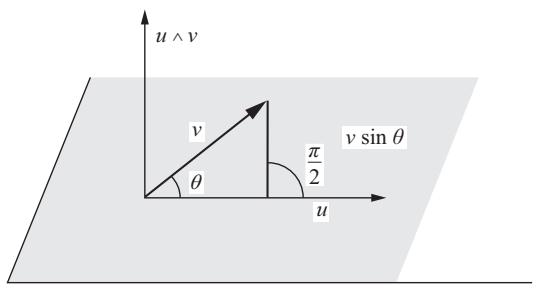
\includegraphics[width=\textwidth]{../../../PDFs/differential-geometry/transcript/Do Carmo - Differential Geometry of Curves and Surfaces/hybrid_ocr/images/184a2a5cb54f57e8b0095aa8826470f2b433badc9f4dadb5c5fb24d76ad02bd1.jpg}}
\end{minipage}
\end{figure}

\begin{Remark}
向量积在曲线理论中的应用：
\begin{itemize}
\item 构造副法向量：$\mathbf{b} = \mathbf{t} \times \mathbf{n}$
\item 计算挠率：$\tau = \dfrac{\det(\alpha', \alpha'', \alpha''')}{k^2}$
\end{itemize}
\end{Remark}

\begin{figure}[H]
\centering
\begin{minipage}{0.6\textwidth}
\centering
\subfloat[Figure 1-12. 弧长逼近的几何意义]{\label{fig:arc-length-approx}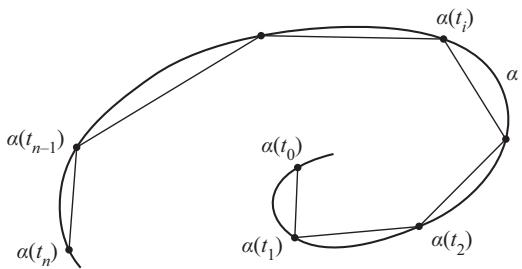
\includegraphics[width=\textwidth]{../../../PDFs/differential-geometry/transcript/Do Carmo - Differential Geometry of Curves and Surfaces/hybrid_ocr/images/a9b16e888308f3816e421a0b7d3bfe30d5b264884d0cead14690e87b887aef3e.jpg}}
\end{minipage}
\end{figure}

\subsection*{1-4 节练习}

\begin{exercise}{1-4, 1 — do Carmo, Exercise 1-4, 1}
Check whether the following bases are positive:
\begin{enumerate}
\item[a.] The basis $\{(1,3),(4,2)\}$ in $\mathbb{R}^2$.
\item[b.] The basis $\{(1,3,5),(2,3,7),(4,8,3)\}$ in $\mathbb{R}^3$.
\end{enumerate}
\end{exercise}

\begin{exercise}{1-4, 2* — do Carmo, Exercise 1-4, 2}
A plane $P$ contained in $\mathbb{R}^3$ is given by the equation $ax + by + cz + d = 0$. Show that the vector $v = (a, b, c)$ is perpendicular to the plane and that $|d| / \sqrt{a^2 + b^2 + c^2}$ measures the distance from the plane to the origin $(0, 0, 0)$.
\end{exercise}

\begin{exercise}{1-4, 3* — do Carmo, Exercise 1-4, 3}
Determine the angle of intersection of the two planes $5x + 3y + 2z - 4 = 0$ and $3x + 4y - 7z = 0$.
\end{exercise}

\begin{exercise}{1-4, 4* — do Carmo, Exercise 1-4, 4}
Given two planes $a_i x + b_i y + c_i z + d_i = 0$, $i = 1, 2$, prove that a necessary and sufficient condition for them to be parallel is
\[
\frac{a_1}{a_2} = \frac{b_1}{b_2} = \frac{c_1}{c_2},
\]
where the convention is made that if a denominator is zero, the corresponding numerator is also zero.
\end{exercise}

\begin{exercise}{1-4, 5 — do Carmo, Exercise 1-4, 5}
Show that an equation of a plane passing through three noncollinear points $p_1 = (x_1, y_1, z_1)$, $p_2 = (x_2, y_2, z_2)$, $p_3 = (x_3, y_3, z_3)$ is given by
\[
(p - p_1) \wedge (p - p_2) \cdot (p - p_3) = 0,
\]
where $p = (x, y, z)$ is an arbitrary point of the plane.
\end{exercise}

\begin{exercise}{1-4, 6* — do Carmo, Exercise 1-4, 6}
Given two nonparallel planes $a_i x + b_i y + c_i z + d_i = 0$, $i = 1, 2$, show that their line of intersection may be parametrized as
\[
x - x_0 = u_1 t, \quad y - y_0 = u_2 t, \quad z - z_0 = u_3 t,
\]
where $(x_0, y_0, z_0)$ belongs to the intersection and $u = (u_1, u_2, u_3)$ is the vector product $u = v_1 \wedge v_2$, $v_i = (a_i, b_i, c_i)$, $i = 1, 2$.
\end{exercise}

\begin{exercise}{1-4, 7* — do Carmo, Exercise 1-4, 7}
Prove that a necessary and sufficient condition for the plane $ax + by + cz + d = 0$ and the line $x - x_0 = u_1 t$, $y - y_0 = u_2 t$, $z - z_0 = u_3 t$ to be parallel is $a u_1 + b u_2 + c u_3 = 0$.
\end{exercise}

\begin{exercise}{1-4, 8* — do Carmo, Exercise 1-4, 8}
Prove that the distance $\rho$ between the nonparallel lines
\[
\begin{array}{l}
x - x_0 = u_1 t, \quad y - y_0 = u_2 t, \quad z - z_0 = u_3 t, \\
x - x_1 = v_1 t, \quad y - y_1 = v_2 t, \quad z - z_1 = v_3 t
\end{array}
\]
is given by
\[
\rho = \frac{|(u \wedge v) \cdot r|}{|u \wedge v|},
\]
where $u = (u_1, u_2, u_3)$, $v = (v_1, v_2, v_3)$, $r = (x_0 - x_1, y_0 - y_1, z_0 - z_1)$.
\end{exercise}

\begin{exercise}{1-4, 9 — do Carmo, Exercise 1-4, 9}
Determine the angle of intersection of the plane $3x + 4y + 7z + 8 = 0$ and the line $x - 2 = 3t$, $y - 3 = 5t$, $z - 5 = 9t$.
\end{exercise}

\begin{exercise}{1-4, 10 — do Carmo, Exercise 1-4, 10}
The natural orientation of $\mathbb{R}^2$ makes it possible to associate a sign to the area $A$ of a parallelogram generated by two linearly independent vectors $u, v \in \mathbb{R}^2$. Show that $A^2 = \left| \begin{smallmatrix} u_1 & u_2 \\ v_1 & v_2 \end{smallmatrix} \right|^2$.
\end{exercise}

\begin{exercise}{1-4, 11 — do Carmo, Exercise 1-4, 11}
\begin{enumerate}
\item[a.] Show that the volume $V$ of a parallelepiped generated by three linearly independent vectors $u, v, w \in \mathbb{R}^3$ is given by $V = |(u \wedge v) \cdot w|$, and introduce an oriented volume in $\mathbb{R}^3$.
\item[b.] Prove that
\[
V^2 = \left| \begin{array}{ccc}
u \cdot u & u \cdot v & u \cdot w \\
v \cdot u & v \cdot v & v \cdot w \\
w \cdot u & w \cdot v & w \cdot w
\end{array} \right|.
\]
\end{enumerate}
\end{exercise}

\begin{exercise}{1-4, 12 — do Carmo, Exercise 1-4, 12}
Given the vectors $v \neq 0$ and $w$, show that there exists a vector $u$ such that $u \wedge v = w$ if and only if $v$ is perpendicular to $w$. Is this vector $u$ uniquely determined? If not, what is the most general solution?
\end{exercise}

\begin{exercise}{1-4, 13 — do Carmo, Exercise 1-4, 13}
Let $u(t) = (u_1(t), u_2(t), u_3(t))$ and $v(t) = (v_1(t), v_2(t), v_3(t))$ be differentiable maps from the interval $(a, b)$ into $\mathbb{R}^3$. If the derivatives $u'(t)$ and $v'(t)$ satisfy the conditions
\[
u'(t) = a u(t) + b v(t), \quad v'(t) = c u(t) - a v(t),
\]
where $a, b$, and $c$ are constants, show that $u(t) \wedge v(t)$ is a constant vector.
\end{exercise}

\begin{exercise}{1-4, 14 — do Carmo, Exercise 1-4, 14}
Find all unit vectors which are perpendicular to the vector $(2, 2, 1)$ and parallel to the plane determined by the points $(0, 0, 0)$, $(1, -2, 1)$, $(-1, 1, 1)$.
\end{exercise}

% ==================== Section 1-5: The Local Theory of Curves ====================
\section{The Local Theory of Curves Parametrized by Arc Length}\label{sec:local-theory-ch1}

\textbf{Answering our original question.} 在引言中，我们提出了一个看似简单却贯穿整个微分几何发展的问题：\textit{如何用精确的数学语言来描述曲线的弯曲程度？}

现在，我们已经有了足够的工具来回答这个问题。回想一下，对于单位速度曲线 $\alpha(s)$，速度向量 $\alpha'(s)$ 是单位切向量。那么，加速度向量 $\alpha''(s)$ 反映了什么？

几何直觉告诉我们：如果曲线是"直的"，那么沿曲线匀速运动的质点没有加速度；如果曲线是"弯曲的"，质点必须承受加速度以改变运动方向。因此，$\alpha''(s)$ 的大小自然就度量了曲线的弯曲程度。这引导我们引入曲率的概念。

\subsection{The Curvature}\label{sec:curvature}

\begin{Definition}[曲率]\label{def:curvature-ch1}
设 $\alpha(s)$ 是单位速度曲线。定义\textbf{曲率}（curvature）为
\[
k(s) = \|\alpha''(s)\|.
\]
即加速度向量的模长。
\end{Definition}

曲率捕捉了曲线弯曲程度的本质。直线的曲率为零——它完全不弯曲。圆的曲率是恒定的 $1/a$（$a$ 为半径）——圆周上每一点的弯曲程度都是均匀的。曲率越大，曲线弯曲得越厉害。

\begin{figure}[H]
\centering
\begin{minipage}{0.6\textwidth}
\centering
\subfloat[Figure 1-14. 曲率的几何意义]{\label{fig:curvature-geom}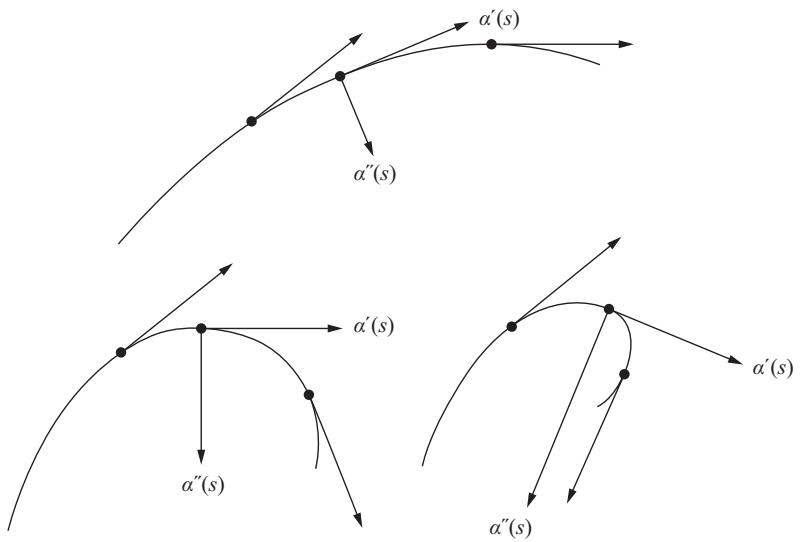
\includegraphics[width=\textwidth]{../../../PDFs/differential-geometry/transcript/Do Carmo - Differential Geometry of Curves and Surfaces/hybrid_ocr/images/1aaf7d0d16f921f25b0f42575a0f8c844242e11985ae269a55e18b4acf7ad5b1.jpg}}
\end{minipage}
\end{figure}

\begin{Example}[圆的曲率]\label{ex:circle-curvature-ch1}
单位圆的参数方程 $\alpha(s) = (\cos s, \sin s, 0)$，则
\[
\alpha'(s) = (-\sin s, \cos s, 0),\quad \alpha''(s) = (-\cos s, -\sin s, 0),
\]
所以 $k(s) = \|\alpha''(s)\| = 1$。更一般地，半径为 $a$ 的圆的曲率为 $1/a$。
\end{Example}

\begin{Example}[直线的曲率]\label{ex:line-curvature-ch1}
直线 $\alpha(s) = \mathbf{p} + \mathbf{v}s$（$\mathbf{v}$ 为单位向量），则 $\alpha''(s) = 0$，所以 $k(s) = 0$。
\end{Example}

\begin{Definition}[主法向量]\label{def:principal-normal}
设 $\alpha(s)$ 是单位速度曲线，$k(s) > 0$。定义\textbf{主法向量}（principal normal）为
\[
\mathbf{n}(s) = \frac{\alpha''(s)}{k(s)} = \frac{\alpha''(s)}{\|\alpha''(s)\|}.
\]
\end{Definition}

\begin{Proposition}[曲率的另一个表达式]\label{prop:curvature-alternative}
设 $\alpha(t)$ 是正则曲线（不一定单位速度），则
\[
k(t) = \frac{\|\alpha'(t) \times \alpha''(t)\|}{\|\alpha'(t)\|^3}.
\]\footnote{推导见附录 \cref{sec:appendix-ch1-curvature-alt}。}
\end{Proposition}

\subsection{The Torsion (Or Bending)}\label{sec:torsion}

\textbf{Beyond curvature.} 曲率已经告诉我们曲线在每一点如何弯曲。然而，这还不够。考虑一个关键问题：给定一条曲线，我们可以找到包含它的最小平面（密切平面）。但如果曲线"扭曲"出这个平面呢？

这种"扭曲"的程度由挠率度量。直观上，如果一条曲线始终位于某个平面内（如圆、椭圆等平面曲线），它就没有扭曲，挠率为零。但如果曲线像螺旋线那样在空间中盘旋，它就会持续"扭转"出每个密切平面——这就是挠率所捕捉的。

挠率描述曲线在空间中的扭曲程度：平面曲线的挠率恒为零（因为 $\alpha', \alpha'', \alpha'''$ 共面），而空间曲线（如螺旋线）的挠率可能非零。

\begin{Definition}[挠率]\label{def:torsion-ch1}
设 $\alpha(s)$ 是单位速度曲线，假设 $k(s) > 0$。定义\textbf{挠率}（torsion）为
\[
\tau(s) = \frac{\det(\alpha'(s), \alpha''(s), \alpha'''(s))}{k(s)^2}.
\]
\end{Definition}

\begin{Remark}
挠率描述曲线在空间中的扭曲程度：
\begin{itemize}
\item 平面曲线：挠率恒为零（因为 $\alpha', \alpha'', \alpha'''$ 共面）；
\item 空间曲线：挠率可能非零，描述曲线"扭转"的程度。
\end{itemize}
\end{Remark}

\begin{Example}[圆柱螺旋线的挠率]\label{ex:helix-torsion-ch1}
圆柱螺旋线 $\alpha(t) = (a\cos t, a\sin t, bt)$ 的曲率为 $k = \dfrac{a}{a^2+b^2}$，挠率为 $\tau = \dfrac{b}{a^2+b^2}$，两者均为常数。
\end{Example}

\begin{Proposition}[挠率的另一个表达式]\label{prop:torsion-alternative}
设 $\alpha(s)$ 是单位速度曲线，$k(s) > 0$，则
\[
\tau(s) = -\langle \mathbf{b}'(s), \mathbf{n}(s) \rangle,
\]
其中 $\mathbf{b}(s) = \mathbf{t}(s) \times \mathbf{n}(s)$ 是副法向量。\footnote{推导见附录 \cref{sec:appendix-ch1-torsion-alt}。}
\end{Proposition}

\begin{figure}[H]
\centering
\begin{minipage}{0.6\textwidth}
\centering
\subfloat[Figure 1-15. 密切平面与 Frenet 标架]{\label{fig:osculating-plane}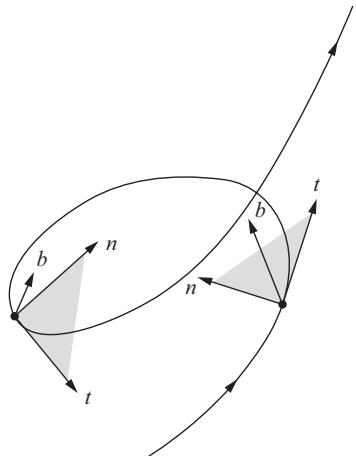
\includegraphics[width=\textwidth]{../../../PDFs/differential-geometry/transcript/Do Carmo - Differential Geometry of Curves and Surfaces/hybrid_ocr/images/df17d953f8624c3870ca864e22d606bcf5467c6aa64274d0f56de41cb925f55b.jpg}}
\end{minipage}
\end{figure}

\subsection{The Frenet-Serret Formulas}\label{sec:frenet-serret}

\textbf{The fundamental theorem.} 给定一个点上的曲率和挠率，我们就知道了曲线在该点的所有几何信息。Frenet-Serret 公式揭示了一个更深层的事实：曲率和挠率不仅决定了曲线的基本性质，而且给定作为弧长函数的光滑曲率 $k(s) > 0$ 和挠率 $\tau(s)$，存在一条（局部意义下的）唯一曲线以之为曲率和挠率。这就是曲线论的基本定理。

这个定理的核心工具是 Frenet 标架——一个随曲线移动的正交标架。

\begin{Definition}[Frenet 标架]\label{def:frenet-frame-ch1}
设 $\alpha(s)$ 是单位速度曲线，$k(s) > 0$。定义：
\begin{enumerate}
\item \textbf{切向量}（tangent vector）：$\mathbf{t}(s) = \alpha'(s)$；
\item \textbf{主法向量}（principal normal）：$\mathbf{n}(s) = \dfrac{\alpha''(s)}{k(s)}$；
\item \textbf{副法向量}（binormal）：$\mathbf{b}(s) = \mathbf{t}(s) \times \mathbf{n}(s)$。
\end{enumerate}
$\{\mathbf{t}, \mathbf{n}, \mathbf{b}\}$ 称为\textbf{Frenet 标架}（Frenet frame）。它们构成 $\mathbb{R}^3$ 的标准正交基（右手系）。
\end{Definition}

\begin{figure}[H]
\centering
\begin{minipage}{0.45\textwidth}
\centering
\subfloat[Figure 1-16 (a). 有向曲率 - 正向]{\label{fig:signed-curvature-pos}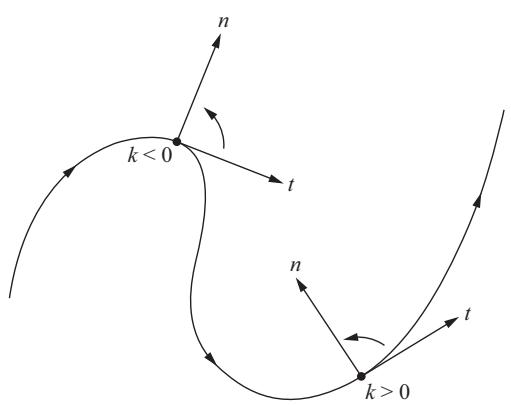
\includegraphics[width=\textwidth]{../../../PDFs/differential-geometry/transcript/Do Carmo - Differential Geometry of Curves and Surfaces/hybrid_ocr/images/55c8df215ceffa70ad05761b78e5c57a32b3796d9d40e2914ae6e471b5f58de1.jpg}}
\end{minipage}
\hfill
\begin{minipage}{0.45\textwidth}
\centering
\subfloat[Figure 1-16 (b). 有向曲率 - 负向]{\label{fig:signed-curvature-neg}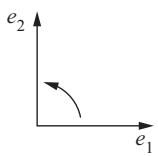
\includegraphics[width=\textwidth]{../../../PDFs/differential-geometry/transcript/Do Carmo - Differential Geometry of Curves and Surfaces/hybrid_ocr/images/857b8e3e7e82e9d09b5e70dd850b1451dc6d837a1b5bdb42717a3c286dd929b6.jpg}}
\end{minipage}
\end{figure}

\begin{Definition}[密切平面、法平面、化直平面]\label{def:osculating-plane-ch1}
\begin{itemize}
\item \textbf{密切平面}（osculating plane）：由 $\mathbf{t}(s)$ 和 $\mathbf{n}(s)$ 张成的平面；
\item \textbf{法平面}（normal plane）：由 $\mathbf{n}(s)$ 和 $\mathbf{b}(s)$ 张成的平面；
\item \textbf{化直平面}（rectifying plane）：由 $\mathbf{t}(s)$ 和 $\mathbf{b}(s)$ 张成的平面。
\end{itemize}
\end{Definition}

\begin{Theorem}[Frenet-Serret 公式]\label{th:frenet-serret-ch1}
设 $\alpha(s)$ 是单位速度曲线，$k(s) > 0$，挠率为 $\tau(s)$。则
\[
\begin{cases}
\mathbf{t}' = k \mathbf{n}, \\
\mathbf{n}' = -k \mathbf{t} + \tau \mathbf{b}, \\
\mathbf{b}' = -\tau \mathbf{n}.
\end{cases}
\]\footnote{直观解释与推导思路见附录 \cref{sec:appendix-ch1-frenet-serret}。}
\end{Theorem}

\begin{Corollary}[曲率和挠率的计算]\label{cor:curvature-torsion-ch1}
曲率和挠率可以通过以下公式计算：
\[
k = \|\mathbf{t}'\|, \quad \tau = -\langle \mathbf{b}', \mathbf{n} \rangle.
\]
\end{Corollary}

\begin{Remark}
Frenet-Serret 公式表明，如果我们知道曲率 $k(s)$ 和挠率 $\tau(s)$，以及初始的 Frenet 标架，就可以唯一确定曲线的形状。这两个函数完全决定了曲线（在局部意义上）。这类似于刚体运动学：给定线速度和角速度，就能确定刚体的运动。
\end{Remark}

\begin{Theorem}[曲线存在唯一性定理]\label{th:curve-existence-ch1}
给定两个连续函数 $k(s) > 0$ 和 $\tau(s)$，以及 $\mathbb{R}^3$ 中一组正交标架，存在唯一一条单位速度曲线 $\alpha(s)$，使得其曲率为 $k(s)$、挠率为 $\tau(s)$，且 Frenet 标架为给定的标架。
\end{Theorem}

\begin{Remark}
这是微分几何中的一个基本存在唯一性定理。它告诉我们：曲率和挠率完全决定了曲线的形状。
\end{Remark}

\begin{figure}[H]
\centering
\begin{minipage}{0.6\textwidth}
\centering
\subfloat[Figure 1-17. 渐伸线 (evolute)]{\label{fig:evolute-ch1}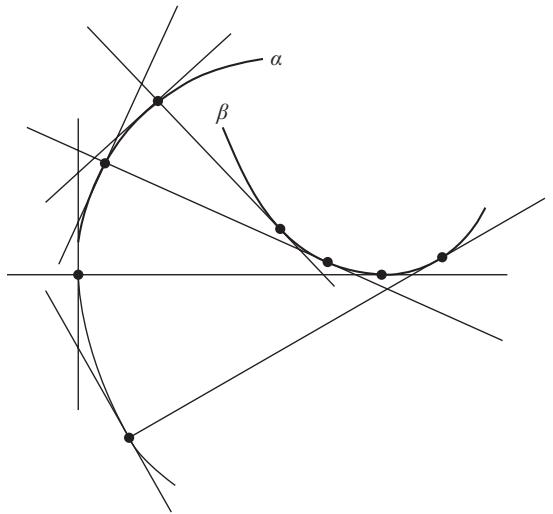
\includegraphics[width=\textwidth]{../../../PDFs/differential-geometry/transcript/Do Carmo - Differential Geometry of Curves and Surfaces/hybrid_ocr/images/85b70efc49d0cda9439f1c08272dfd6fec2be67d419e7c9bbdd49d8b9c082da6.jpg}}
\end{minipage}
\end{figure}

\subsection*{1-5 节练习}

除非特别说明，$\alpha: \mathbf{I} \to \mathbf{R}^3$ 是单位速度曲线，曲率 $k(s) \neq 0$。

\begin{exercise}{1-5, 1 — do Carmo, Exercise 1-5, 1}
Given the parametrized curve (helix)
\[
\alpha(s) = \left(a\cos\frac{s}{c}, a\sin\frac{s}{c}, b\frac{s}{c}\right), \quad s \in \mathbb{R},
\]
where $c^2 = a^2 + b^2$,
\begin{enumerate}
\item[a.] Show that the parameter $s$ is the arc length.
\item[b.] Determine the curvature and the torsion of $\alpha$.
\item[c.] Determine the osculating plane of $\alpha$.
\item[d.] Show that the lines containing $n(s)$ and passing through $\alpha(s)$ meet the $z$ axis under a constant angle equal to $\pi/2$.
\item[e.] Show that the tangent lines to $\alpha$ make a constant angle with the $z$ axis.
\end{enumerate}
\end{exercise}

\begin{exercise}{1-5, 2* — do Carmo, Exercise 1-5, 2}
Show that the torsion $\tau$ of $\alpha$ is given by
\[
\tau(s) = - \frac{\alpha'(s) \wedge \alpha''(s) \cdot \alpha'''(s)}{|k(s)|^2}.
\]
\end{exercise}

\begin{exercise}{1-5, 3 — do Carmo, Exercise 1-5, 3}
Assume that $\alpha(I) \subset \mathbb{R}^2$ (i.e., $\alpha$ is a plane curve) and give $k$ a sign. Transport the vectors $t(s)$ parallel to themselves so that the origins of $t(s)$ agree with the origin of $\mathbb{R}^2$; the end points of $t(s)$ then describe a parametrized curve $s \to t(s)$ called the indicatrix of tangents of $\alpha$. Let $\theta(s)$ be the angle from $e_1$ to $t(s)$ in the orientation of $\mathbb{R}^2$. Prove:
\begin{enumerate}
\item[a.] The indicatrix of tangents is a regular parametrized curve.
\item[b.] $dt/ds = (d\theta/ds)n$, that is, $k = d\theta/ds$.
\end{enumerate}
\end{exercise}

\begin{exercise}{1-5, 4* — do Carmo, Exercise 1-5, 4}
Assume that all normals of a parametrized curve pass through a fixed point. Prove that the trace of the curve is contained in a circle.
\end{exercise}

\begin{exercise}{1-5, 5 — do Carmo, Exercise 1-5, 5}
A regular parametrized curve $\alpha$ has the property that all its tangent lines pass through a fixed point.
\begin{enumerate}
\item[a.] Prove that the trace of $\alpha$ is a (segment of a) straight line.
\item[b.] Does the conclusion in part a still hold if $\alpha$ is not regular?
\end{enumerate}
\end{exercise}

\begin{exercise}{1-5, 6 — do Carmo, Exercise 1-5, 6}
A translation by a vector $v$ in $\mathbb{R}^3$ is the map $A: \mathbb{R}^3 \to \mathbb{R}^3$ that is given by $A(p) = p + v$, $p \in \mathbb{R}^3$. A linear map $\rho: \mathbb{R}^3 \to \mathbb{R}^3$ is an orthogonal transformation when $\rho u \cdot \rho v = u \cdot v$ for all vectors $u, v \in \mathbb{R}^3$. A rigid motion in $\mathbb{R}^3$ is the result of composing a translation with an orthogonal transformation with positive determinant.
\begin{enumerate}
\item[a.] Demonstrate that the norm of a vector and the angle $\theta$ between two vectors, $0 \leq \theta \leq \pi$, are invariant under orthogonal transformations with positive determinant.
\item[b.] Show that the vector product of two vectors is invariant under orthogonal transformations with positive determinant. Is the assertion still true if we drop the condition on the determinant?
\item[c.] Show that the arc length, the curvature, and the torsion of a parametrized curve are (whenever defined) invariant under rigid motions.
\end{enumerate}
\end{exercise}

\begin{exercise}{1-5, 7* — do Carmo, Exercise 1-5, 7}
Let $\alpha: I \to \mathbb{R}^2$ be a regular parametrized plane curve (arbitrary parameter), and define $n = n(t)$ and $k = k(t)$. Assume that $k(t) \neq 0$, $t \in I$. In this situation, the curve
\[
\beta(t) = \alpha(t) + \frac{1}{k(t)} n(t), \quad t \in I,
\]
is called the \textbf{evolute} of $\alpha$ (渐伸线，教材 Figure 1-17（见 \cref{fig:evolute-ch1}）).
\begin{enumerate}
\item[a.] Show that the tangent at $t$ of the evolute of $\alpha$ is the normal to $\alpha$ at $t$.
\item[b.] Consider the normal lines of $\alpha$ at two neighboring points $t_1, t_2$, $t_1 \neq t_2$. Let $t_1$ approach $t_2$ and show that the intersection points of the normals converge to a point on the trace of the evolute of $\alpha$.
\end{enumerate}
\end{exercise}

\begin{exercise}{1-5, 8 — do Carmo, Exercise 1-5, 8}
The trace of the parametrized curve (arbitrary parameter)
\[
\alpha(t) = (t, \cosh t), \quad t \in \mathbb{R},
\]
is called the \textbf{catenary} (悬链线).
\begin{enumerate}
\item[a.] Show that the signed curvature of the catenary is
\[
k(t) = \frac{1}{\cosh^2 t}.
\]
\item[b.] Show that the evolute of the catenary is
\[
\beta(t) = (t - \sinh t \cosh t, 2\cosh t).
\]
\end{enumerate}
\end{exercise}

\begin{exercise}{1-5, 9 — do Carmo, Exercise 1-5, 9}
Given a differentiable function $k(s)$, $s \in I$, show that the parametrized plane curve having $k(s) = k$ as curvature is given by
\[
\alpha(s) = \left(\int \cos\theta(s) ds + a, \int \sin\theta(s) ds + b\right),
\]
where
\[
\theta(s) = \int k(s) ds + \varphi,
\]
and that the curve is determined up to a translation of the vector $(a, b)$ and a rotation of the angle $\varphi$.
\end{exercise}

\begin{exercise}{1-5, 10 — do Carmo, Exercise 1-5, 10}
Consider the map
\[
\alpha(t) = \begin{cases}
(t, 0, e^{-1/t^2}), & t > 0, \\
(t, e^{-1/t^2}, 0), & t < 0, \\
(0, 0, 0), & t = 0.
\end{cases}
\]
\begin{enumerate}
\item[a.] Prove that $\alpha$ is a differentiable curve.
\item[b.] Prove that $\alpha$ is regular for all $t$ and that the curvature $k(t) \neq 0$, for $t \neq 0, t \neq \pm\sqrt{2/3}$, and $k(0) = 0$.
\item[c.] Show that the limit of the osculating planes as $t \to 0$, $t > 0$, is the plane $y = 0$ but that the limit of the osculating planes as $t \to 0$, $t < 0$, is the plane $z = 0$ (this implies that the normal vector is discontinuous at $t = 0$ and shows why we excluded points where $k = 0$).
\item[d.] Show that $\tau$ can be defined so that $\tau \equiv 0$, even though $\alpha$ is not a plane curve.
\end{enumerate}
\end{exercise}

\begin{exercise}{1-5, 11 — do Carmo, Exercise 1-5, 11}
One often gives a plane curve in polar coordinates by $\rho = \rho(\theta)$, $a \leq \theta \leq b$.
\begin{enumerate}
\item[a.] Show that the arc length is
\[
\int_a^b \sqrt{\rho^2 + (\rho')^2} d\theta,
\]
where the prime denotes the derivative relative to $\theta$.
\item[b.] Show that the curvature is
\[
k(\theta) = \frac{2(\rho')^2 - \rho\rho'' + \rho^2}{\{(\rho')^2 + \rho^2\}^{3/2}}.
\]
\end{enumerate}
\end{exercise}

\begin{exercise}{1-5, 12* — do Carmo, Exercise 1-5, 12}
Let $\alpha: I \to \mathbb{R}^3$ be a regular parametrized curve (not necessarily by arc length) and let $\beta: J \to \mathbb{R}^3$ be a reparametrization of $\alpha(I)$ by the arc length $s = s(t)$, measured from $t_0 \in I$. Let $t = t(s)$ be the inverse function of $s$ and set $d\alpha/dt = \alpha'$, $d^2\alpha/dt^2 = \alpha''$, etc. Prove:
\begin{enumerate}
\item[a.] $dt/ds = 1/|\alpha'|$, $d^2t/ds^2 = -(\alpha' \cdot \alpha'' / |\alpha'|^4)$.
\item[b.] The curvature of $\alpha$ at $t \in I$ is
\[
k(t) = \frac{|\alpha' \wedge \alpha''|}{|\alpha'|^3}.
\]
\item[c.] The torsion of $\alpha$ at $t \in I$ is
\[
\tau(t) = - \frac{(\alpha' \wedge \alpha'') \cdot \alpha'''}{|\alpha' \wedge \alpha''|^2}.
\]
\item[d.] If $\alpha: I \to \mathbb{R}^2$ is a plane curve $\alpha(t) = (x(t), y(t))$, the signed curvature of $\alpha$ at $t$ is
\[
k(t) = \frac{x'y'' - x''y'}{((x')^2 + (y')^2)^{3/2}}.
\]
\end{enumerate}
\end{exercise}

\begin{exercise}{1-5, 13* — do Carmo, Exercise 1-5, 13}
Assume that $\tau(s) \neq 0$ and $k'(s) \neq 0$ for all $s \in I$. Show that a necessary and sufficient condition for $\alpha(I)$ to lie on a sphere is that
\[
R^2 + (R')^2 T^2 = \mathrm{const.},
\]
where $R = 1/k$, $T = 1/\tau$, and $R'$ is the derivative of $R$ relative to $s$.
\end{exercise}

\begin{exercise}{1-5, 14 — do Carmo, Exercise 1-5, 14}
Let $\alpha: (a, b) \to \mathbb{R}^2$ be a regular parametrized plane curve. Assume that there exists $t_0$, $a < t_0 < b$, such that the distance $|\alpha(t)|$ from the origin to the trace of $\alpha$ will be a maximum at $t_0$. Prove that the curvature $k$ of $\alpha$ at $t_0$ satisfies $|k(t_0)| \geq 1/|\alpha(t_0)|$.
\end{exercise}

\begin{exercise}{1-5, 15* — do Carmo, Exercise 1-5, 15}
Show that the knowledge of the vector function $b = b(s)$ (binormal vector) of a curve $\alpha$, with nonzero torsion everywhere, determines the curvature $k(s)$ and the absolute value of the torsion $\tau(s)$ of $\alpha$.
\end{exercise}

\begin{exercise}{1-5, 16* — do Carmo, Exercise 1-5, 16}
Show that the knowledge of the vector function $n = n(s)$ (normal vector) of a curve $\alpha$, with nonzero torsion everywhere, determines the curvature $k(s)$ and the torsion $\tau(s)$ of $\alpha$.
\end{exercise}

\begin{exercise}{1-5, 17 — do Carmo, Exercise 1-5, 17}
In general, a curve $\alpha$ is called a \textbf{helix} if the tangent lines of $\alpha$ make a constant angle with a fixed direction. Assume that $\tau(s) \neq 0$, $s \in I$, and prove that:
\begin{enumerate}
\item[a.] $\alpha$ is a helix if and only if $k/\tau = \mathrm{const}$.
\item[b.] $\alpha$ is a helix if and only if the lines containing $n(s)$ and passing through $\alpha(s)$ are parallel to a fixed plane.
\item[c.*] $\alpha$ is a helix if and only if the lines containing $b(s)$ and passing through $\alpha(s)$ make a constant angle with a fixed direction.
\item[d.] The curve
\[
\alpha(s) = \left(\frac{a}{c}\int\sin\theta(s) ds, \frac{a}{c}\int\cos\theta(s) ds, \frac{b}{c}s\right),
\]
where $c^2 = a^2 + b^2$, is a helix, and that $k/\tau = a/b$.
\end{enumerate}
\end{exercise}

\begin{exercise}{1-5, 18* — do Carmo, Exercise 1-5, 18}
Let $\alpha: I \to \mathbb{R}^3$ be a parametrized regular curve (not necessarily by arc length) with $k(t) \neq 0$, $\tau(t) \neq 0$, $t \in I$. The curve $\alpha$ is called a \textbf{Bertrand curve} if there exists a curve $\bar{\alpha}: I \to \mathbb{R}^3$ such that the normal lines of $\alpha$ and $\bar{\alpha}$ at $t \in I$ are equal. In this case, $\bar{\alpha}$ is called a \textbf{Bertrand mate} of $\alpha$, and we can write
\[
\bar{\alpha}(t) = \alpha(t) + r n(t).
\]
Prove that:
\begin{enumerate}
\item[a.] $r$ is constant.
\item[b.] $\alpha$ is a Bertrand curve if and only if there exists a linear relation
\[
Ak(t) + B\tau(t) = 1, \quad t \in I,
\]
where $A, B$ are nonzero constants and $k$ and $\tau$ are the curvature and torsion of $\alpha$, respectively.
\item[c.] If $\alpha$ has more than one Bertrand mate, it has infinitely many Bertrand mates. This case occurs if and only if $\alpha$ is a circular helix.
\end{enumerate}
\end{exercise}

% ==================== Section 1-6: The Local Canonical Form ====================
\section{The Local Canonical Form}\label{sec:local-canonical-form-ch1}

本节研究曲线在一点附近的局部形状。

\begin{Theorem}[曲线在一点的局部标准形式]\label{th:local-canonical-form-ch1}
设 $\alpha(s)$ 是以弧长 $s$ 为参数的可微曲线，在 $s = s_0$ 处 $k(s_0) > 0$。则
\[
\alpha(s) = \alpha(s_0) + (s - s_0)\mathbf{t}_0 + \frac{(s - s_0)^2}{2}k_0\mathbf{n}_0 + \frac{(s - s_0)^3}{6}k_0\tau_0\mathbf{b}_0 + o((s - s_0)^3),
\]
其中 $\mathbf{t}_0 = \mathbf{t}(s_0)$，$k_0 = k(s_0)$，$\tau_0 = \tau(s_0)$。
\end{Theorem}

\begin{Remark}
这个展开式揭示了曲线的几何意义：
\begin{itemize}
\item 线性项 $(s - s_0)\mathbf{t}_0$：沿切方向 $\mathbf{t}$ 的运动；
\item 二次项 $\dfrac{(s - s_0)^2}{2}k_0\mathbf{n}_0$：沿法方向 $\mathbf{n}$ 的弯曲（由曲率 $k$ 控制）；
\item 三次项 $\dfrac{(s - s_0)^3}{6}k_0\tau_0\mathbf{b}_0$：沿副法方向 $\mathbf{b}$ 的扭曲（由挠率 $\tau$ 控制）。
\end{itemize}
\end{Remark}

\begin{Remark}
当 $\tau(s_0) = 0$ 但 $k(s_0) \neq 0$ 时，曲线在 $s_0$ 附近是平面曲线（因为三次项为零）。
\end{Remark}

\begin{Definition}[密切圆]\label{def:osculating-circle-ch1}
曲线在 $s_0$ 处的\textbf{密切圆}（osculating circle）是半径为 $1/k(s_0)$、圆心在 $\alpha(s_0) + \dfrac{1}{k(s_0)}\mathbf{n}(s_0)$ 的圆。
\end{Definition}

\begin{Remark}
密切圆与曲线在切点有相同的切方向和曲率。它是曲线在该点附近最好的圆近似。
\end{Remark}

\begin{figure}[H]
\centering
\begin{minipage}{0.45\textwidth}
\centering
\subfloat[Figure 1-18. 局部标准形式的投影]{\label{fig:local-canonical-projections}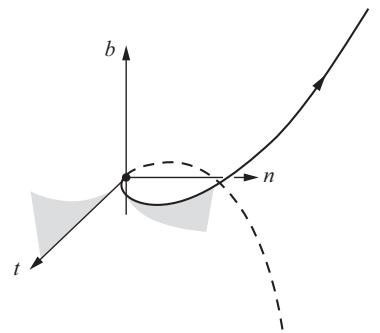
\includegraphics[width=\textwidth]{../../../PDFs/differential-geometry/transcript/Do Carmo - Differential Geometry of Curves and Surfaces/hybrid_ocr/images/1e6a547641b1e28e3c702fb6e34f46c8a858b466f072c85a849afa6b33da9d72.jpg}}
\end{minipage}
\hfill
\begin{minipage}{0.45\textwidth}
\centering
\subfloat[投影到 $tb$ 平面]{\label{fig:local-canonical-tb}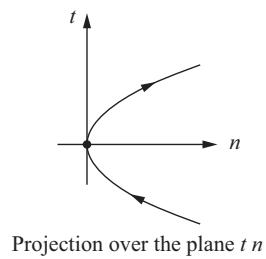
\includegraphics[width=\textwidth]{../../../PDFs/differential-geometry/transcript/Do Carmo - Differential Geometry of Curves and Surfaces/hybrid_ocr/images/559bd128ff198b162ce66c9ee7c9a939cc608cb17870f0e37b55f457b9d26c95.jpg}}
\end{minipage}
\end{figure}

\begin{figure}[H]
\centering
\begin{minipage}{0.45\textwidth}
\centering
\subfloat[投影到 $nb$ 平面]{\label{fig:local-canonical-nb}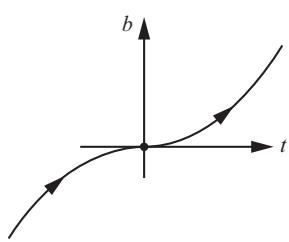
\includegraphics[width=\textwidth]{../../../PDFs/differential-geometry/transcript/Do Carmo - Differential Geometry of Curves and Surfaces/hybrid_ocr/images/1889978426007c61cdf45a97ae5a1a5a5accffabdac10b46b3f8f73f04ef5f86.jpg}}
\end{minipage}
\hfill
\begin{minipage}{0.45\textwidth}
\centering
\subfloat[投影到 $tn$ 平面]{\label{fig:local-canonical-tn}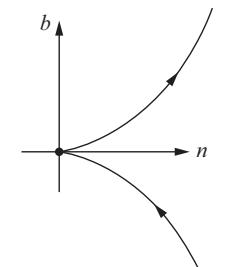
\includegraphics[width=\textwidth]{../../../PDFs/differential-geometry/transcript/Do Carmo - Differential Geometry of Curves and Surfaces/hybrid_ocr/images/1fb0809e26dc4c3d9b71f6f2f4f516ba37417a1ad2f25349083242b67d20e8fe.jpg}}
\end{minipage}
\end{figure}

\begin{figure}[H]
\centering
\begin{minipage}{0.45\textwidth}
\centering
\subfloat[Figure 1-19 (a). $\tau < 0$ 的情形]{\label{fig:torsion-neg}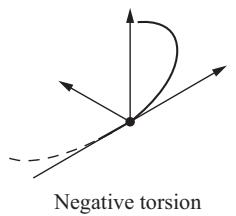
\includegraphics[width=\textwidth]{../../../PDFs/differential-geometry/transcript/Do Carmo - Differential Geometry of Curves and Surfaces/hybrid_ocr/images/5c650a1fbbf8575a4560f36765774966e5be5ecf980eb69ea5bf1c8af1192924.jpg}}
\end{minipage}
\hfill
\begin{minipage}{0.45\textwidth}
\centering
\subfloat[Figure 1-19 (b). $\tau > 0$ 的情形]{\label{fig:torsion-pos}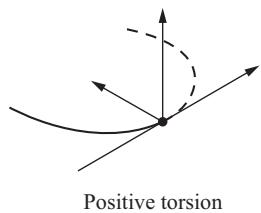
\includegraphics[width=\textwidth]{../../../PDFs/differential-geometry/transcript/Do Carmo - Differential Geometry of Curves and Surfaces/hybrid_ocr/images/44e707e5ada16aaa4e24604909275fc9a43532bcc6a0e1eebde0ea453c90fee0.jpg}}
\end{minipage}
\end{figure}

\subsection*{1-6 节练习}

\begin{exercise}{1-6, 1 — do Carmo, Exercise 1-6, 1}
Let $\alpha: I \to \mathbb{R}^3$ be a curve parametrized by arc length with curvature $k(s) \neq 0$, $s \in I$. Let $P$ be a plane satisfying both of the following conditions:
\begin{enumerate}
\item $P$ contains the tangent line at $s$.
\item Given any neighborhood $J \subset I$ of $s$, there exist points of $\alpha(J)$ in both sides of $P$.
\end{enumerate}
Prove that $P$ is the osculating plane of $\alpha$ at $s$.
\end{exercise}

\begin{exercise}{1-6, 2 — do Carmo, Exercise 1-6, 2}
Let $\alpha: I \to \mathbb{R}^3$ be a curve parametrized by arc length, with curvature $k(s) \neq 0$, $s \in I$. Show that:
\begin{enumerate}
\item[a.] The osculating plane at $s$ is the limit position of the plane passing through $\alpha(s)$, $\alpha(s + h_1)$, $\alpha(s + h_2)$ when $h_1, h_2 \to 0$.
\item[b.] The limit position of the circle passing through $\alpha(s)$, $\alpha(s + h_1)$, $\alpha(s + h_2)$ when $h_1, h_2 \to 0$ is a circle in the osculating plane at $s$, the center of which is on the line that contains $n(s)$ and the radius of which is the radius of curvature $1/k(s)$; this circle is called the osculating circle at $s$.
\end{enumerate}
\end{exercise}

\begin{exercise}{1-6, 3 — do Carmo, Exercise 1-6, 3}
Show that the curvature $k(t) \neq 0$ of a regular parametrized curve $\alpha: I \to \mathbb{R}^3$ is the curvature at $t$ of the plane curve $\pi \circ \alpha$, where $\pi$ is the normal projection of $\alpha$ over the osculating plane at $t$.
\end{exercise}

% ==================== Section 1-7: Global Properties of Plane Curves ====================
\section{Global Properties of Plane Curves}\label{sec:global-properties-ch1}

\textbf{From local to global.} 到目前为止，我们研究的是曲线的\textbf{局部性质}——那些仅依赖于曲线在一点附近行为的几何量。曲率和挠率正是这样的局部不变量。

然而，局部几何并不能告诉我们曲线的全部故事。一条简单闭曲线（如椭圆）与一条自交曲线（如打结的曲线）在每一点都有良好的曲率，但它们的整体形状截然不同。本节中，我们将看到曲线的全局拓扑如何影响其几何性质。

这一主题体现了微分几何的一个核心思想：\textbf{局部性质与整体性质之间的深刻联系}。

\begin{Definition}[简单闭曲线]\label{def:simple-closed-curve}
一条平面曲线 $\alpha: [0, L] \to \mathbb{R}^2$ 称为\textbf{简单闭曲线}（simple closed curve），如果 $\alpha(0) = \alpha(L)$，且 $\alpha$ 在 $(0, L)$ 上是单射。
\end{Definition}

简单闭曲线是平面曲线中最自然的闭合曲线——它不自交，像一条橡皮筋首尾相接。

\begin{figure}[H]
\centering
\begin{minipage}{0.45\textwidth}
\centering
\subfloat[Figure 1-20 (a). 简单闭曲线]{\label{fig:simple-closed}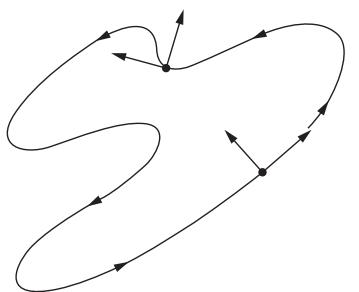
\includegraphics[width=\textwidth]{../../../PDFs/differential-geometry/transcript/Do Carmo - Differential Geometry of Curves and Surfaces/hybrid_ocr/images/8ea4e8eea7678cad3948cf06b0551ceecf71afff5bf72bb6f76985d606f4722b.jpg}}
\end{minipage}
\hfill
\begin{minipage}{0.45\textwidth}
\centering
\subfloat[Figure 1-20 (b). 非简单闭曲线]{\label{fig:nonsimple-closed}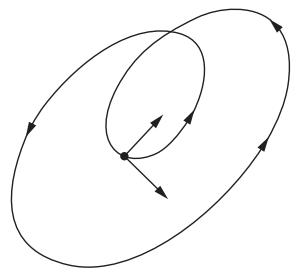
\includegraphics[width=\textwidth]{../../../PDFs/differential-geometry/transcript/Do Carmo - Differential Geometry of Curves and Surfaces/hybrid_ocr/images/034960a7cc6b6fde35352465512e26d15cc4232f9875e588aab42f7e9fe01290.jpg}}
\end{minipage}
\end{figure}

\begin{figure}[H]
\centering
\begin{minipage}{0.45\textwidth}
\centering
\subfloat[Figure 1-21 (a). 环面上的简单闭曲线]{\label{fig:torus-curve}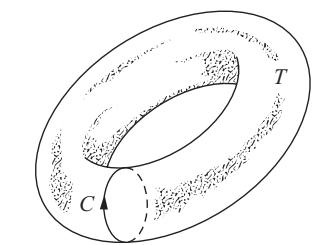
\includegraphics[width=\textwidth]{../../../PDFs/differential-geometry/transcript/Do Carmo - Differential Geometry of Curves and Surfaces/hybrid_ocr/images/3a2b0c77969ff7631fc9d313f3e38b0d4d65257a4b99a9b9ca75b8e5446ee999.jpg}}
\end{minipage}
\hfill
\begin{minipage}{0.45\textwidth}
\centering
\subfloat[Figure 1-21 (b). 正向定向]{\label{fig:positive-orientation}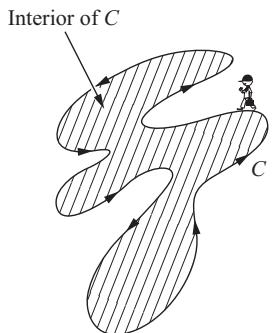
\includegraphics[width=\textwidth]{../../../PDFs/differential-geometry/transcript/Do Carmo - Differential Geometry of Curves and Surfaces/hybrid_ocr/images/d1fa06b0b42dfa82fca2be8e907ef38765cb5fdc93c76d29bcda32a65eb9f15c.jpg}}
\end{minipage}
\end{figure}

\begin{Definition}[旋转指数]\label{def:turning-number-ch1}
设 $\alpha: [0, L] \to \mathbb{R}^2$ 是一条简单闭平面曲线，参数化为单位速度。定义\textbf{旋转指数}（turning number）为
\[
n = \frac{1}{2\pi} \int_0^L k(s) \, ds.
\]
旋转指数表示切向量沿曲线完整一圈转过的圈数。
\end{Definition}

旋转指数是一个优雅的概念：它将曲率（局部几何量）沿曲线积分，得到一个与全局拓扑相关的整数。

\begin{Theorem}[旋转指数定理]\label{th:turning-number}
简单闭平面曲线的旋转指数必为整数，且绝对值至少为 $1$。
\end{Theorem}

这个定理揭示了一个惊人事实：无论曲线的形状多么复杂，其切向量旋转的"总圈数"必然是整数。这类似于经典力学中转动一周角度必为 $2\pi$ 的整数倍。

\begin{Theorem}[四顶点定理]\label{th:four-vertex-ch1}
设 $C$ 是平面上一条简单闭曲线，曲率恒为正。则 $C$ 上至少有四个曲率极值点（顶点）。
\end{Theorem}

"顶点"（vertex）是指曲率取得局部极值的点。四顶点定理是平面曲线理论中最著名的整体定理之一——它告诉我们，任意一条简单闭曲线的曲率不能只有一个峰值，必须"起伏"至少四次。椭圆恰好有四个顶点（长轴和短轴的端点）。

\begin{Theorem}[Fenchel 定理]\label{th:fenchel-ch1}
设 $\alpha: [0, L] \to \mathbb{R}^3$ 是一条简单闭曲线。则其全曲率
\[
\int_0^L k(s) \, ds \geq 2\pi,
\]
等号成立当且仅当曲线是平面上的凸曲线。
\end{Theorem}

\textbf{Why does this matter?} Fenchel 定理告诉我们一个令人惊讶的事实：无论一条闭曲线如何在空间中扭曲、打结，它沿自身的"总弯曲量"至少是 $2\pi$。这就像是说，无论你如何弯曲一根绳子再将其首尾相连，这根绳子弯曲的总量必然不少于整好绕一圈所需的弯曲。

\begin{Definition}[全曲率]\label{def:total-curvature-ch1}
曲线 $\alpha$ 的\textbf{全曲率}（total curvature）定义为
\[
\int_0^L k(s) \, ds,
\]
即曲率沿曲线的积分。
\end{Definition}

\begin{Corollary}\label{cor:fenchel-corollary-ch1}
任何简单闭曲线的全曲率至少为 $2\pi$。
\end{Corollary}

\begin{Theorem}[Fary-Milnor 定理]\label{th:fary-milnor-ch1}
如果 $\alpha$ 是一条简单闭曲线的全曲率小于 $4\pi$，则该曲线是未打结的（unknotted）。
\end{Theorem}

Fary-Milnor 定理更进了一步：如果总弯曲量小于 $4\pi$，这根"绳子"就打不成结。这建立了曲线的整体拓扑（能否打结）与局部几何量（曲率积分）之间的深刻联系。

\begin{figure}[H]
\centering
\begin{minipage}{0.65\textwidth}
\centering
\subfloat[Figure 1-22. 等周公式证明图示]{\label{fig:fig1-22}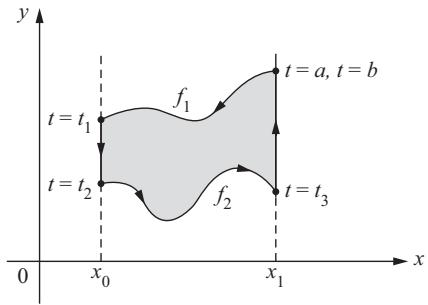
\includegraphics[width=\textwidth]{../../../PDFs/differential-geometry/transcript/Do Carmo - Differential Geometry of Curves and Surfaces/hybrid_ocr/images/9cfc830e55606447f8926843d144db8601ec13fc42473572cd665be08fc2c5e7.jpg}}
\end{minipage}
\end{figure}

\begin{figure}[H]
\centering
\begin{minipage}{0.45\textwidth}
\centering
\subfloat[Figure 1-23. 等周问题的几何构型]{\label{fig:isoperimetric-config}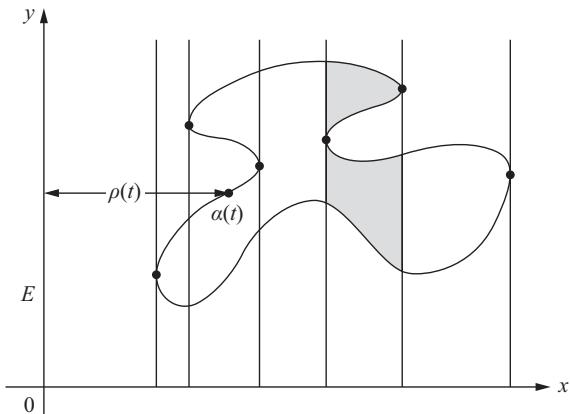
\includegraphics[width=\textwidth]{../../../PDFs/differential-geometry/transcript/Do Carmo - Differential Geometry of Curves and Surfaces/hybrid_ocr/images/29ac0046be9d030e2d6b0d51c57778a994e77f9712ebe5ac2a3e63401941f75b.jpg}}
\end{minipage}
\hfill
\begin{minipage}{0.45\textwidth}
\centering
\subfloat[Figure 1-24. 等周不等式证明图示]{\label{fig:isoperimetric-proof}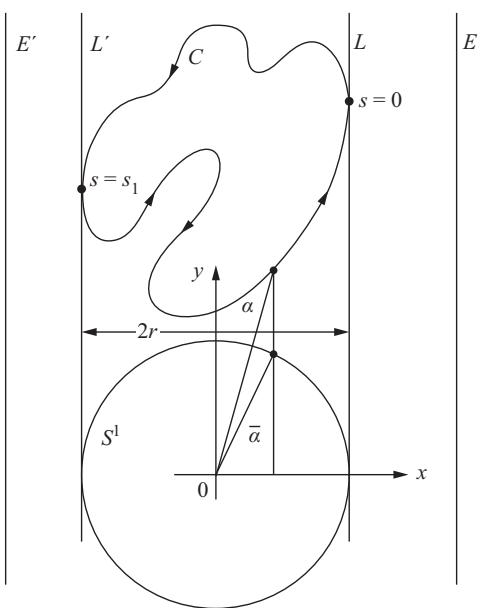
\includegraphics[width=\textwidth]{../../../PDFs/differential-geometry/transcript/Do Carmo - Differential Geometry of Curves and Surfaces/hybrid_ocr/images/1f888342851bea2237ad4ebb2ceefdc9cdeca51246d624ddcbad61b94698552a.jpg}}
\end{minipage}
\end{figure}

\begin{figure}[H]
\centering
\begin{minipage}{0.6\textwidth}
\centering
\subfloat[Figure 1-25. 分段 $C^1$ 曲线]{\label{fig:piecewise-c1}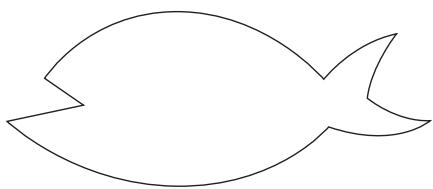
\includegraphics[width=\textwidth]{../../../PDFs/differential-geometry/transcript/Do Carmo - Differential Geometry of Curves and Surfaces/hybrid_ocr/images/a325c45e4316d76cdb849939f3c5c8e59eeabe101ad105b382b0edef3e23eec6.jpg}}
\end{minipage}
\end{figure}

\begin{figure}[H]
\centering
\begin{minipage}{0.45\textwidth}
\centering
\subfloat[Figure 1-26 (a). 切线指标线]{\label{fig:tangent-indicatrix-a}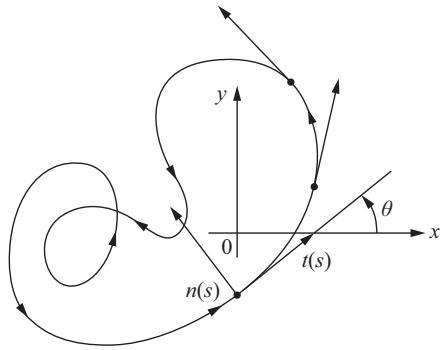
\includegraphics[width=\textwidth]{../../../PDFs/differential-geometry/transcript/Do Carmo - Differential Geometry of Curves and Surfaces/hybrid_ocr/images/ed8972f41acdd947228696eb1aff57a22d3c79ea04195b25322152a5092b2d99.jpg}}
\end{minipage}
\hfill
\begin{minipage}{0.45\textwidth}
\centering
\subfloat[Figure 1-26 (b). 切线指标线详图]{\label{fig:tangent-indicatrix-b}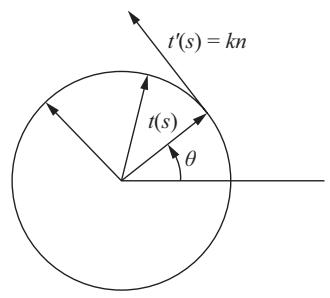
\includegraphics[width=\textwidth]{../../../PDFs/differential-geometry/transcript/Do Carmo - Differential Geometry of Curves and Surfaces/hybrid_ocr/images/9f5cb3a1ae7c39a5420c6e25848ff8d26636e1a07af4c18bf87cb74dcb14f23d.jpg}}
\end{minipage}
\end{figure}

\begin{figure}[H]
\centering
\begin{minipage}{0.45\textwidth}
\centering
\subfloat[Figure 1-27 (a). 旋转指数为 1]{\label{fig:rotation-index-1}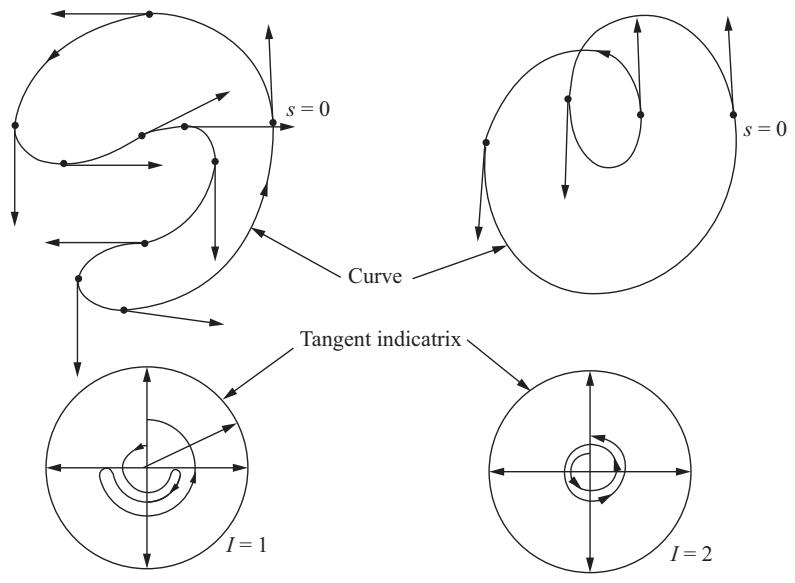
\includegraphics[width=\textwidth]{../../../PDFs/differential-geometry/transcript/Do Carmo - Differential Geometry of Curves and Surfaces/hybrid_ocr/images/c1056d2b6a48d0190f210c9a7fdeba0fa262e8791d59f8252ee8a071b806c76f.jpg}}
\end{minipage}
\hfill
\begin{minipage}{0.45\textwidth}
\centering
\subfloat[Figure 1-27 (b). 旋转指数为 2]{\label{fig:rotation-index-2}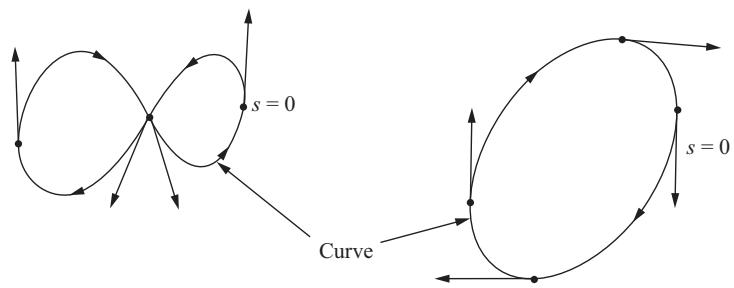
\includegraphics[width=\textwidth]{../../../PDFs/differential-geometry/transcript/Do Carmo - Differential Geometry of Curves and Surfaces/hybrid_ocr/images/bfcd46a1040027336d83edcb81d47775141684cb0bba7c3dda59703c841db26b.jpg}}
\end{minipage}
\end{figure}

\begin{figure}[H]
\centering
\begin{minipage}{0.80\textwidth}
\centering
\subfloat[Figure 1-27 (c). 旋转指数为 -1]{\label{fig:rotation-index-neg}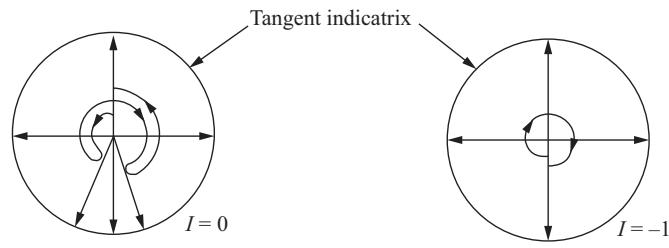
\includegraphics[width=\textwidth]{../../../PDFs/differential-geometry/transcript/Do Carmo - Differential Geometry of Curves and Surfaces/hybrid_ocr/images/4344fb6535e6e590751cfcb71fc7a04ab9c88b236c3504c6bb25fafcfc9c5319.jpg}}
\end{minipage}
\end{figure}

\begin{figure}[H]
\centering
\begin{minipage}{0.75\textwidth}
\centering
\subfloat[Figure 1-28 (a). 凸曲线]{\label{fig:convex-curve}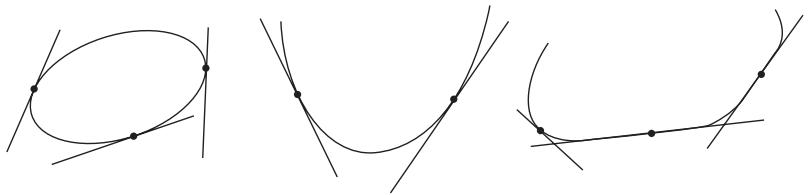
\includegraphics[width=\textwidth]{../../../PDFs/differential-geometry/transcript/Do Carmo - Differential Geometry of Curves and Surfaces/hybrid_ocr/images/605b716c932cd5e915b8e5296bc4b3e577a93f4c7d7d3fc35e7590742cd5296c.jpg}}
\end{minipage}
\end{figure}

\begin{figure}[H]
\centering
\begin{minipage}{0.70\textwidth}
\centering
\subfloat[Figure 1-28 (b). 非凸曲线]{\label{fig:nonconvex-curve}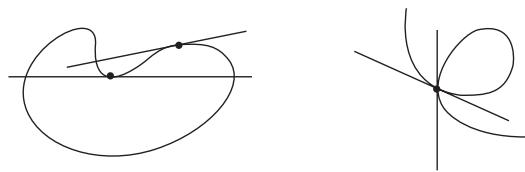
\includegraphics[width=\textwidth]{../../../PDFs/differential-geometry/transcript/Do Carmo - Differential Geometry of Curves and Surfaces/hybrid_ocr/images/344549a18768464cdc807bdd43ffa550bccfb9852fa5b59672c3d2e70141e497.jpg}}
\end{minipage}
\end{figure}

\begin{figure}[H]
\centering
\begin{minipage}{0.35\textwidth}
\centering
\subfloat[Figure 1-29 (a). 三个不同顶点情况]{\label{fig:four-vertex-a}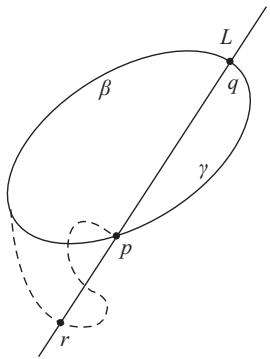
\includegraphics[width=\textwidth]{../../../PDFs/differential-geometry/transcript/Do Carmo - Differential Geometry of Curves and Surfaces/hybrid_ocr/images/2797eca07f5b8cd6e2426a408534d07b5f1671cf8aa13f28a1b57bab08ecd395.jpg}}
\end{minipage}
\end{figure}

\begin{figure}[H]
\centering
\begin{minipage}{0.85\textwidth}
\centering
\subfloat[Figure 1-29 (b). 直线段情况]{\label{fig:four-vertex-b}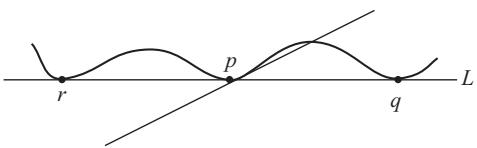
\includegraphics[width=\textwidth]{../../../PDFs/differential-geometry/transcript/Do Carmo - Differential Geometry of Curves and Surfaces/hybrid_ocr/images/ce7874597bf7b56abe143614c8510607de566ea4819d497bea3b17078bf3fa4f.jpg}}
\end{minipage}
\end{figure}

\begin{figure}[H]
\centering
\begin{minipage}{0.6\textwidth}
\centering
\subfloat[Figure 1-30. 直线族的重数]{\label{fig:line-multiplicity}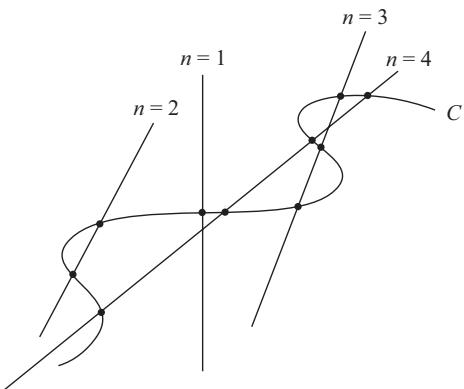
\includegraphics[width=\textwidth]{../../../PDFs/differential-geometry/transcript/Do Carmo - Differential Geometry of Curves and Surfaces/hybrid_ocr/images/8af60fc93ea0ea82b08ce868637d63a5a839095d24f97b10ab057990e28d0abd.jpg}}
\end{minipage}
\end{figure}

\begin{figure}[H]
\centering
\begin{minipage}{0.6\textwidth}
\centering
\subfloat[Figure 1-31. 直线的参数化]{\label{fig:line-param}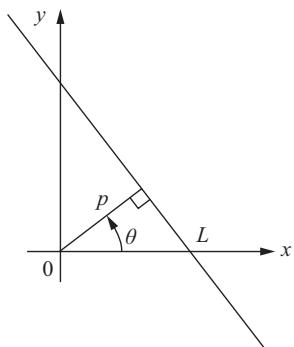
\includegraphics[width=\textwidth]{../../../PDFs/differential-geometry/transcript/Do Carmo - Differential Geometry of Curves and Surfaces/hybrid_ocr/images/cd4f1bfb9e7c57e2454775fece77bc5393aca16227f9e880341f8709494dea67.jpg}}
\end{minipage}
\end{figure}

\begin{figure}[H]
\centering
\begin{minipage}{0.6\textwidth}
\centering
\subfloat[Figure 1-32. 刚体运动]{\label{fig:rigid-motion}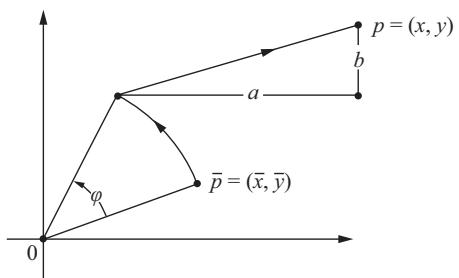
\includegraphics[width=\textwidth]{../../../PDFs/differential-geometry/transcript/Do Carmo - Differential Geometry of Curves and Surfaces/hybrid_ocr/images/8623bd4bd41d13ccfa7b56b4da654a8467c435e3d691498e94a601f3dafb2ae8.jpg}}
\end{minipage}
\end{figure}

\subsection*{1-7 节练习}

\begin{exercise}{1-7, 1* — do Carmo, Exercise 1-7, 1}
Is there a simple closed curve in the plane with length equal to 6 feet and bounding an area of 3 square feet?
\end{exercise}

\begin{exercise}{1-7, 2* — do Carmo, Exercise 1-7, 2}
Let $\overline{AB}$ be a segment of straight line and let $l > \text{length of } AB$. Show that the curve $C$ joining $A$ and $B$, with length $l$, and such that together with $\overline{AB}$ bounds the largest possible area is an arc of a circle passing through $A$ and $B$ (教材 Figure 1-23（见 \cref{fig:isoperimetric-config}）、Figure 1-24（见 \cref{fig:isoperimetric-proof}）)。
\end{exercise}

\begin{exercise}{1-7, 3 — do Carmo, Exercise 1-7, 3}
Compute the curvature of the ellipse $x = a\cos t$, $y = b\sin t$, $t \in [0, 2\pi]$, $a \neq b$, and show that it has exactly four vertices, namely, $(a, 0)$, $(-a, 0)$, $(0, b)$, $(0, -b)$.
\end{exercise}

\begin{exercise}{1-7, 4* — do Carmo, Exercise 1-7, 4}
Let $C$ be a plane curve and let $T$ be the tangent line at a point $p \in C$. Draw a line $L$ parallel to the normal line at $p$ and at a distance $d$ of $p$. Let $h$ be the length of the segment determined on $L$ by $C$ and $T$. Prove that $|k(p)| = \lim_{d \to 0} \frac{2h}{d^2}$.
\end{exercise}

\begin{exercise}{1-7, 5* — do Carmo, Exercise 1-7, 5}
If a closed plane curve $C$ is contained inside a disk of radius $r$, prove that there exists a point $p \in C$ such that the curvature $k$ of $C$ at $p$ satisfies $|k| \geq 1/r$.
\end{exercise}

\begin{exercise}{1-7, 6 — do Carmo, Exercise 1-7, 6}
Let $\alpha(s)$, $s \in [0, l]$ be a closed convex plane curve positively oriented. The curve $\beta(s) = \alpha(s) - r\mathbf{n}(s)$, where $r$ is a positive constant and $\mathbf{n}$ is the normal vector, is called a parallel curve to $\alpha$. Show that:
\begin{enumerate}
\item[a.] Length of $\beta = $ length of $\alpha + 2\pi r$.
\item[b.] $A(\beta) = A(\alpha) + rl + \pi r^2$.
\item[c.] $k_\beta(s) = k_\alpha(s) / (1 + r k_\alpha(s))$.
\end{enumerate}
\end{exercise}

\begin{exercise}{1-7, 7 — do Carmo, Exercise 1-7, 7}
Let $\alpha: \mathbb{R} \to \mathbb{R}^2$ be a plane curve defined in the entire real line. Assume that $\alpha$ does not pass through the origin and that both $\lim_{t \to +\infty} |\alpha(t)| = \infty$ and $\lim_{t \to -\infty} |\alpha(t)| = \infty$.
\begin{enumerate}
\item[a.] Prove that there exists a point $t_0 \in \mathbb{R}$ such that $|\alpha(t_0)| \leq |\alpha(t)|$ for all $t \in \mathbb{R}$.
\item[b.] Show, by an example, that the assertion in part a is false if one does not assume both limits are infinite.
\end{enumerate}
\end{exercise}

\begin{exercise}{1-7, 8* — do Carmo, Exercise 1-7, 8}
\begin{enumerate}
\item[a.] Let $\alpha(s)$, $s \in [0, l]$, be a plane simple closed curve. Assume that the curvature $k(s)$ satisfies $0 < k(s) \leq c$. Prove that $\text{length of } \alpha \geq 2\pi/c$.
\item[b.] In part a replace the assumption of being simple by "$\alpha$ has rotation index $N$". Prove that $\text{length of } \alpha \geq 2\pi N/c$.
\end{enumerate}
\end{exercise}

\begin{exercise}{1-7, 9* — do Carmo, Exercise 1-7, 9}
A set $K \subset \mathbb{R}^2$ is convex if given any two points $p, q \in K$ the segment of straight line $\overline{pq}$ is contained in $K$ (教材 Figure 1-38（见 \cref{fig:fig1-38}）). Prove that a simple closed convex curve bounds a convex set.
\end{exercise}

\begin{exercise}{1-7, 10 — do Carmo, Exercise 1-7, 10}
Let $C$ be a convex plane curve. Prove geometrically that $C$ has no self-intersections.
\end{exercise}

\begin{exercise}{1-7, 11* — do Carmo, Exercise 1-7, 11}
Given a nonconvex simple closed plane curve $C$, we can consider its convex hull $H$ (教材 Figure 1-39（见 \cref{fig:fig1-39}）). Use this to show that, in the isoperimetric problem, we can restrict ourselves to convex curves.
\end{exercise}

\begin{exercise}{1-7, 12* — do Carmo, Exercise 1-7, 12}
Consider a unit circle $S^1$ in the plane. Show that the ratio $M_1/M_2 = 1/2$, where $M_2$ is the measure of the set of straight lines in the plane that meet $S^1$ and $M_1$ is the measure of all such lines that determine in $S^1$ a chord of length $> \sqrt{3}$ (教材 Figure 1-40（见 \cref{fig:fig1-40}）)。
\end{exercise}

\begin{exercise}{1-7, 13 — do Carmo, Exercise 1-7, 13}
Let $C$ be an oriented plane closed curve with curvature $k > 0$. Assume that $C$ has at least one point $p$ of self-intersection. Prove that:
\begin{enumerate}
\item[a.] There is a point $p' \in C$ such that the tangent line $T'$ at $p'$ is parallel to some tangent at $p$.
\item[b.] The rotation angle of the tangent in the positive arc of $C$ made up by $pp'p$ is $> \pi$ (教材 Figure 1-41（见 \cref{fig:fig1-41}）)。
\item[c.] The rotation index of $C$ is $\geq 2$.
\end{enumerate}
\end{exercise}

\begin{exercise}{1-7, 14 — do Carmo, Exercise 1-7, 14}
\begin{enumerate}
\item[a.] Show that if a straight line $L$ meets a closed convex curve $C$, then either $L$ is tangent to $C$ or $L$ intersects $C$ in exactly two points.
\item[b.] Use part a to show that the measure of the set of lines that meet $C$ (without multiplicities) is equal to the length of $C$.
\end{enumerate}
\end{exercise}

\begin{exercise}{1-7, 15 — do Carmo, Exercise 1-7, 15}
Green's theorem in the plane: Let a simple closed plane curve be given by $\alpha(t) = (x(t), y(t))$, $t \in [a, b]$. Assume that $\alpha$ is positively oriented, let $C$ be its trace, and let $R$ be the interior of $C$. Let $p = p(x, y)$, $q = q(x, y)$ be real functions. Then
\[
\iint_R (q_x - p_y) \, dx \, dy = \int_C (p \, dx + q \, dy).
\]
\begin{enumerate}
\item[a.] Set $q = x$ and $p = -y$ and conclude that $A(R) = \frac{1}{2} \int_a^b (x \, dy - y \, dx) \, dt$.
\item[b.] Use Green's theorem to obtain the transformation formula for double integrals.
\end{enumerate}
\end{exercise}

\begin{figure}[H]
\centering
\begin{minipage}{0.3\textwidth}
\centering
\subfloat[Figure 1-38. 凸集定义]{\label{fig:fig1-38}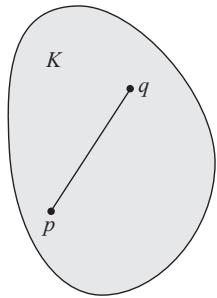
\includegraphics[width=\textwidth]{../../../PDFs/differential-geometry/transcript/Do Carmo - Differential Geometry of Curves and Surfaces/hybrid_ocr/images/291667aa35426f0fc1ad84813595a255703e09fa4939bf88cba52c32fffc50c4.jpg}}
\end{minipage}
\hfill
\begin{minipage}{0.3\textwidth}
\centering
\subfloat[Figure 1-39. 凸包]{\label{fig:fig1-39}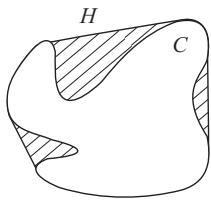
\includegraphics[width=\textwidth]{../../../PDFs/differential-geometry/transcript/Do Carmo - Differential Geometry of Curves and Surfaces/hybrid_ocr/images/3e78224695b6747abf33b1b0932df3f39b60339272bb783ed8d858be5aadb2c6.jpg}}
\end{minipage}
\hfill
\begin{minipage}{0.35\textwidth}
\centering
\subfloat[Figure 1-40. 单位圆与等边三角形]{\label{fig:fig1-40}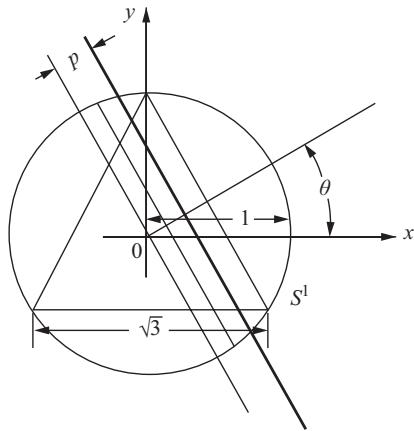
\includegraphics[width=\textwidth]{../../../PDFs/differential-geometry/transcript/Do Carmo - Differential Geometry of Curves and Surfaces/hybrid_ocr/images/00ec3ddff9ad514cf917444fd074562155a12997a49a644f7ec0989cf7e7d2e8.jpg}}
\end{minipage}
\end{figure}

\begin{figure}[H]
\centering
\begin{minipage}{0.55\textwidth}
\centering
\subfloat[Figure 1-41. 自交曲线旋转角]{\label{fig:fig1-41}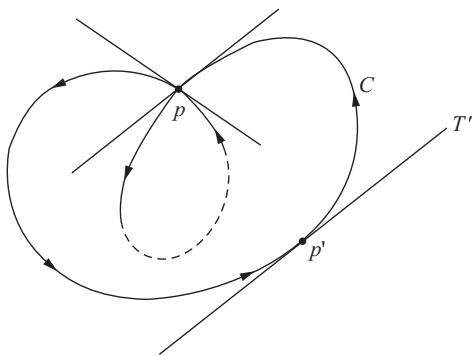
\includegraphics[width=\textwidth]{../../../PDFs/differential-geometry/transcript/Do Carmo - Differential Geometry of Curves and Surfaces/hybrid_ocr/images/196b87ce5dc9f30daed335b19890a1abf143cb5ea589b33a25641998f788084a.jpg}}
\end{minipage}
\end{figure}

\endinput
